\documentclass{scrreprt}
\usepackage[latin1]{inputenc}
\usepackage[spanish]{babel}
\usepackage{listings}
\usepackage{underscore}
\usepackage{tabularx}
\usepackage[bookmarks=true]{hyperref}
\usepackage{framed}
\usepackage[section]{placeins}
\usepackage{graphicx}
\usepackage{adjustbox}
\usepackage{etoolbox}
\usepackage{ifthen}
\usepackage{array}
\newcolumntype{L}{>{\centering\arraybackslash}m{3cm}}
\hypersetup{
    pdftitle={Especificaci�n de requisitos de software},    % title
    pdfauthor={autores},                     % author
    pdfsubject={TeX and LaTeX},                        % subject of the document
    pdfkeywords={TeX, LaTeX, graphics, images}, % list of keywords
    colorlinks=true,       % false: boxed links; true: colored links
    linkcolor=blue,       % color of internal links
    citecolor=black,       % color of links to bibliography
    filecolor=black,        % color of file links
    urlcolor=purple,        % color of external links
    linktoc=page            % only page is linked
}%
\def\myversion{1.0 }
\title{%
\flushright
\rule{16cm}{5pt}\vskip1cm
\Huge{ESPECIFICACI�N DE REQUISITOS DE\\SOFTWARE}\\
\vspace{2cm}
para\\
\vspace{1.7cm}
Librer�a de Software Interna\\
\vspace{1.7cm}
\LARGE{Entrega 1.0\\}
\vspace{1.7cm}
\LARGE{Version \myversion en proceso de aprobaci�n\\}
\vspace{1.7cm}
Preparado por Reinaldo Jer�z,\\Daniela Paredes, Erik Regla y Yorch Sep�lveda\\
\vfill
\rule{16cm}{5pt}
}
\date{}
\newcommand{\reqdescription}[1]{
\phantom{line break}
\par
\noindent\resizebox{\linewidth}{!}{%
\begin{tabularx}{\textwidth}{X}
\textbf{Descripci�n: } #1
\end{tabularx}%
}%
\par
}

\newcommand{\reqrationale}[1]{
\phantom{line break}
\par
\noindent\resizebox{\linewidth}{!}{%
\begin{tabularx}{\textwidth}{X}
\textbf{Raz�n/Motivo: } #1
\end{tabularx}%
}%
\par
}

\newcommand{\reqsource}[1]{
\phantom{line break}
\par
\noindent\resizebox{\linewidth}{!}{%
\begin{tabularx}{\textwidth}{X}
\textbf{Fuente: } #1
\end{tabularx}%
}%
\par
}

\newcommand{\reqfitcriterion}[1]{
\phantom{line break}
\par
\noindent\resizebox{\linewidth}{!}{%
\begin{tabularx}{\textwidth}{X}
\textbf{Criterio de ajuste: } #1
\end{tabularx}%
}%
\par
}

\newcommand{\reqsatisfaction}[2]{
\phantom{line break}
\par
\noindent\resizebox{\linewidth}{!}{%
\begin{tabularx}{\textwidth}{XX}
\textbf{Satisfacci�n del consumidor: } #1 & \textbf{Insatisfacci�n del consumidor: } #2
\end{tabularx}%
}%
\par
}

\newcommand{\reqdepencies}[2]{
\phantom{line break}
\par
\noindent\resizebox{\linewidth}{!}{%
\begin{tabularx}{\textwidth}{XX}
\textbf{Dependencias: } #1 & \textbf{Conflictos: } #2
\end{tabularx}%
}%
\par
}

\newcommand{\reqdocuments}[1]{
\phantom{line break}
\par
\noindent\resizebox{\linewidth}{!}{%
\begin{tabularx}{\textwidth}{X}
\textbf{Documentos: } #1
\end{tabularx}%
}%
\par
}

\newcommand{\reqhistory}[1]{
\phantom{line break}
\par
\noindent\resizebox{\linewidth}{!}{%
\begin{tabularx}{\textwidth}{X}
\textbf{Historial de cambios: } #1
\end{tabularx}%
}%
\par
}
\newcounter{frcounter}%[section]
\newcounter{nfrcounter}%[section]
\newcounter{urcounter}%[section]

\BeforeBeginEnvironment{requirement}{\vspace{0.5cm}\begin{minipage}{\linewidth}}
\AfterEndEnvironment{requirement}{\end{minipage}\par\vspace{0.5cm}}

\newenvironment{requirement}[2]{
\begin{framed}
\ifstrequal{#1}{functional}{\refstepcounter{frcounter}}{%
\ifstrequal{#1}{nonfunctional}{\refstepcounter{nfrcounter}}{%
\refstepcounter{urcounter}}}
\noindent\resizebox{\linewidth}{!}{%
\begin{tabularx}{\textwidth}{X X X}
\textbf{Requisito\#:} %
\ifstrequal{#1}{functional}{RF\thefrcounter}{%
\ifstrequal{#1}{nonfunctional}{RNF\thenfrcounter}{%
RSC\theurcounter}} %
& \textbf{Tipo:} %
\ifthenelse{\equal{#1}{functional}}{Funcional}{%
\ifthenelse{\equal{#1}{nonfunctional}}{No funcional}{}%
}%
& \textbf{Casos de uso: } #2 
\end{tabularx}%
}%
\par
}{\FloatBarrier\end{framed}}

\newcommand{\reffr}[1]{
RF\ref{#1}
}
\newcommand{\refnfr}[1]{
RNF\ref{#1}
}
\newcommand{\refur}[1]{
RSC\ref{#1}
}

\begin{document}
\maketitle
\tableofcontents
%\chapter*{Revision History}
\chapter{Introducci�n}
Muchos alumnos desarrollan proyectos durante su ``vida �til'' en la universidad y estos se pierden debido a que la plataforma utilizada para subirlos (Educandus) no almacena registros de estos trabajos. A causa de esto, las labores de difusi�n llevadas a cabo por la direcci�n de escuela no pueden utilizar esta informaci�n para actividades de pasant�a (como actualmente realiza la escuela de Ingenier�a Civil Industrial).

Adicionalmente al problema de mostrar una cara visible al exterior de la escuela, los profesores no tienen como darle continuidad a proyectos desarrollados durante los m�dulos de formaci�n disciplinar y mucho menos un m�todo �gil de poder seleccionar un proyecto en base a una etapa de avance para planificar un curso de desarrollo de software. 
\chapter{Prop�sito del proyecto}

%\section{El negocio del cliente}
%Nuestro cliente es Rodrigo Bustamante quien es el actual administrador del laboratorio turing. Actualmente se encarga de

\section{Metas del proyecto}
\begin{enumerate}
\item{Tener un registro persistente de software generado dentro de la escuela por alumnos y profesores junto a una documentaci�n comprensiva de estos. De esta manera mejorar el desempe�o de alumnos y profesores dentro de la escuela}
\item{Generar una ``cara visible'' de la escuela hacia el medio, y as� poder mostrar a potenciales alumnos las actividades, artefactos y avances de alumnos de la carrera, mejorando el proceso de difusi�n de la carrera.}

\end{enumerate}


\chapter{Los actores}
% \begin{enumerate}
% \item{\emph{Profesores}}
% \item{\emph{Administradores}}
% \item{\emph{Moderadores}}
% \item{\emph{Alumnos}}
% \item{\emph{Funcionarios}}
% \item{\emph{Personas ajenas a la organizaci�n}}
% \end{enumerate}


\section{Clientes e inversores}
\begin{enumerate}
\item{\emph{Escuela de ingenier�a civil en computaci�n}: 

Actualmente est� enfrentando un serio problema de organizaci�n con 
la informaci�n generada por los alumnos y profesores en temas de 
proyectos desarrollados a lo largo de los cursos} 
A lo largo de la carrera se generan muchos productos por los alumnos, estos productos no tienen un lugar establecido
donde ser almacenados, sino que cada profesor a cargo se encarga de guardarlos de manera aut�noma y con el tiempo estos
terminan desapareciendo. El problema aqu� es que todos esos productos realizados son una ventana que muestra los trabajos
que se realizan durante el curso de la carrera, lo cual perfectamente puede servir para dar a conocer el �mbito de la carrera, como podr�a ser
para investigaciones o como fuente de informaci�n en general.

%\item{\emph{Ruth Garrido}} %ingrese motivos
\end{enumerate}


\section{Consumidores}
\begin{enumerate}
\item{\emph{Profesores}}
Hace referencia a los profesores de la universidad en general, mas espec�ficamente profesores
de la Escuela de Ingenier�a Civil en Computaci�n.
Los profesores de la escuela utilizaran el producto tanto para un tema pedag�gico, como para
obtener informaci�n para investigaciones, adem�s, tendr�n la posibilidad de guardar los productos
realizados en cada modulo para su posterioridad o continuidad en otros cursos.
\item{\emph{Alumnos}}
Hace referencia a alumnos de pregrado u otro nivel de la Universidad de Talca en general.
Los alumnos utilizaran el producto como fuente de conocimiento, pudiendo tomar el material existente
para su continuidad o pudiendo colocar sus propios materiales realizados en los distintos m�dulos.
\item{\emph{Funcionarios}}
Hace referencia a funcionarios de la Universidad de Talca en general.
Los funcionarios en general tambi�n pueden hacer uso de este producto, por ejemplo, funcionarios del �rea
de publicidad podr�an tomar proyectos terminados o proyectos interesantes y mostrarlos al p�blico de manera expl�cita.
Por otra parte, los moderadores y administradores que requerir� el producto no necesariamente deben ser profesores
y pueden ser personas capacitadas que se dediquen a otra �rea dentro de la universidad.
\item{\emph{Personas ajenas a la organizaci�n}}
Este producto no solo se centra en personas de la Universidad, sino tambi�n en personas de afuera. Cualquier persona
ser� capaz de ver y probar proyectos p�blicos, esto juega un doble rol, adem�s de ser una fuente de conocimiento, es un atractivo 
que la universidad presenta a externos que podr�an tomar la calidad de estudiantes alg�n d�a.
\end{enumerate}


\section{Otros inversores}


%ninguno por el momento%
\section{Usuarios finales}
\begin{enumerate}
\item{\emph{Profesores}}
\item{\emph{Alumnos}}
\item{\emph{Directora de escuela}}
Cabe destacar que si bien, la directora puede no entrar en contacto directo con el sistema, este le
beneficia de manera proporcional, dado que, el producto presenta un gran nivel de exposici�n del trabajo realizado durante la carrera
y esto genera un incentivo extra en personas pensando en iniciar una carrera universitaria del �rea (Publicidad y Atracci�n)
\item{\emph{Personas ajenas a la organizaci�n}}
\end{enumerate}
%ruth


\section{Personas}
\begin{enumerate}
\item{\emph{Directora de escuela que busca mostrar proyectos a pasantes}}
\item{\emph{Futuro estudiante de ICC}}
\item{\emph{Alumno que busca documentaci�n de proyectos similares}}
\item{\emph{Pasante curioso de los trabajos realizados en ICC}}
\item{\emph{Tesista que busca trabajos similares realizados previamente}}
\item{\emph{Tesista que entrega su memoria y desea dejar su proyecto en l�nea disponible al p�blico}}
\item{\emph{Alumno que termina un proyecto y se desea subir a la plataforma}}
\item{\emph{Profesor que busca elegir el \textit{starting point} para un curso de ingenier�a de software}}
\item{\emph{Investigador que busca \textit{material} de asistencia}}
\end{enumerate}

\section{Prioridades asignadas a los usuarios}
\begin{enumerate}
\item{\emph{Profesores}}
\item{\emph{Alumnos}}
\item{\emph{Directora de escuela}}
\item{\emph{Personas ajenas a la organizaci�n}}
\end{enumerate}

\section{Participaci�n de los usuarios}
\begin{enumerate}
\item{\emph{Profesores}}
\item{\emph{Alumnos}}
\item{\emph{Directora de escuela}}
\item{\emph{Personas ajenas a la organizaci�n}}
\end{enumerate}

\section{Personal de mantenci�n y t�cnicos}
\begin{enumerate}
\item{\emph{Administradores}}
Los administradores se dedican a controlar los proyectos que son subidos al sistema, 
estos se preocupan de revisar la integridad de estos conforme a las normas establecidas
y posteriormente a aceptarlos o rechazarlos seg�n corresponda. Adem�s de esto, se dedica a procesar
las solicitudes de registro de usuarios, verificando la afiliaci�n a la universidad y la veracidad
de los datos en general, procediendo posteriormente a rechazar la solicitud o aceptarla seg�n corresponda al caso.
Por otra parte tienen como labor gestionar categor�as y etiquetas, enti�ndase por gestionar agregar/modificar/eliminar.
Por �ltimo, tambi�n les corresponde configurar la virtualizaci�n de los proyectos que contengan un paquete ejecutable, 
esto lo realizan segun la documentaci�n entregada en cada proyecto y de manera particular para cada uno. (Adem�s pueden realizar funciones de moderaci�n)
\item{\emph{Moderadores}}
Los moderadores se preocupan de evaluar los comentarios realizados en cada proyecto, esto a fin de evitar
Comentarios fuera de l�nea o que atenten de manera negativa contra los proyectos, lectores o personas participantes.
Adem�s pueden agregar filtros de palabras universales que el sistema aplicara de forma autom�tica.
\end{enumerate} 



\chapter{Restricciones del proyecto}
\section{Restricciones de la soluci�n}
%formas de que el problema puede ser resuelto.
\begin{itemize}
  \item El proyecto debe ser enviado con el c�digo fuente, la documentaci�n, el ejecutable y la descripci�n del proyecto.
  \item Un proyecto no puede ser modificado despu�s de ser aceptado.
  \item Un comentario no puede ser modificado posterior a su moderaci�n.
  \item Una cuenta de usuario no puede ser eliminada pero si deshabilitada.
  \item Un proyecto publicado no puede ser eliminado.
  \item No existe un lapsus de tiempo fijo para subir proyectos.
  \item El idioma del producto es espa�ol.
  \item El sistema debe contar con un control de acceso.
  \item El proyecto no puede contar con un control de versiones.
\end{itemize}

\section{Ambiente de implementaci�n de la soluci�n}
%entorno f�sico y tecnol�gico en el que el producto ser� instalado.
\begin{itemize}
  \item El producto debe ser multiplataforma %(Roa dijo: El producto es una aplicaci�n web)
  \item El formato de compresi�n de los archivos a subir a un proyecto debe ser est�ndar (rar, tar, zip).
\end{itemize}

\section{Aplicaciones colaboradoras o relacionadas}
%aplicaciones que no son parte del producto pero que el producto va a colaborar

\section{Software fuera del alcance}
%aplicaciones que pueden ser usadas para implementar alguno de los requisitos.
%\section{Entorno Anticipado de Trabajo}
%\section{Restricciones de agenda}
%\section{Restricciones de presupuesto}
\section{Restricciones de la organizaci�n}
%nose que va ac� :c

%\chapter{Convenci�n de nombres y terminolog�a}
%\chapter{Hechos relevantes y supuestos}
%\section{Hechos relevantes}
%\section{Reglas del negocio}
%\section{Supuestos}
%\begin{enumerate}
%\item Asumimos que cuando el administrador elimina una cuenta de usuario, tambi�n se eliminan sus proyectos asociados. 
%\end{enumerate}

\chapter{Alcances del trabajo}
\section{Situaci�n actual}
%no hay nada similar
\section{Contexto del trabajo}
\begin{figure}[!ht]
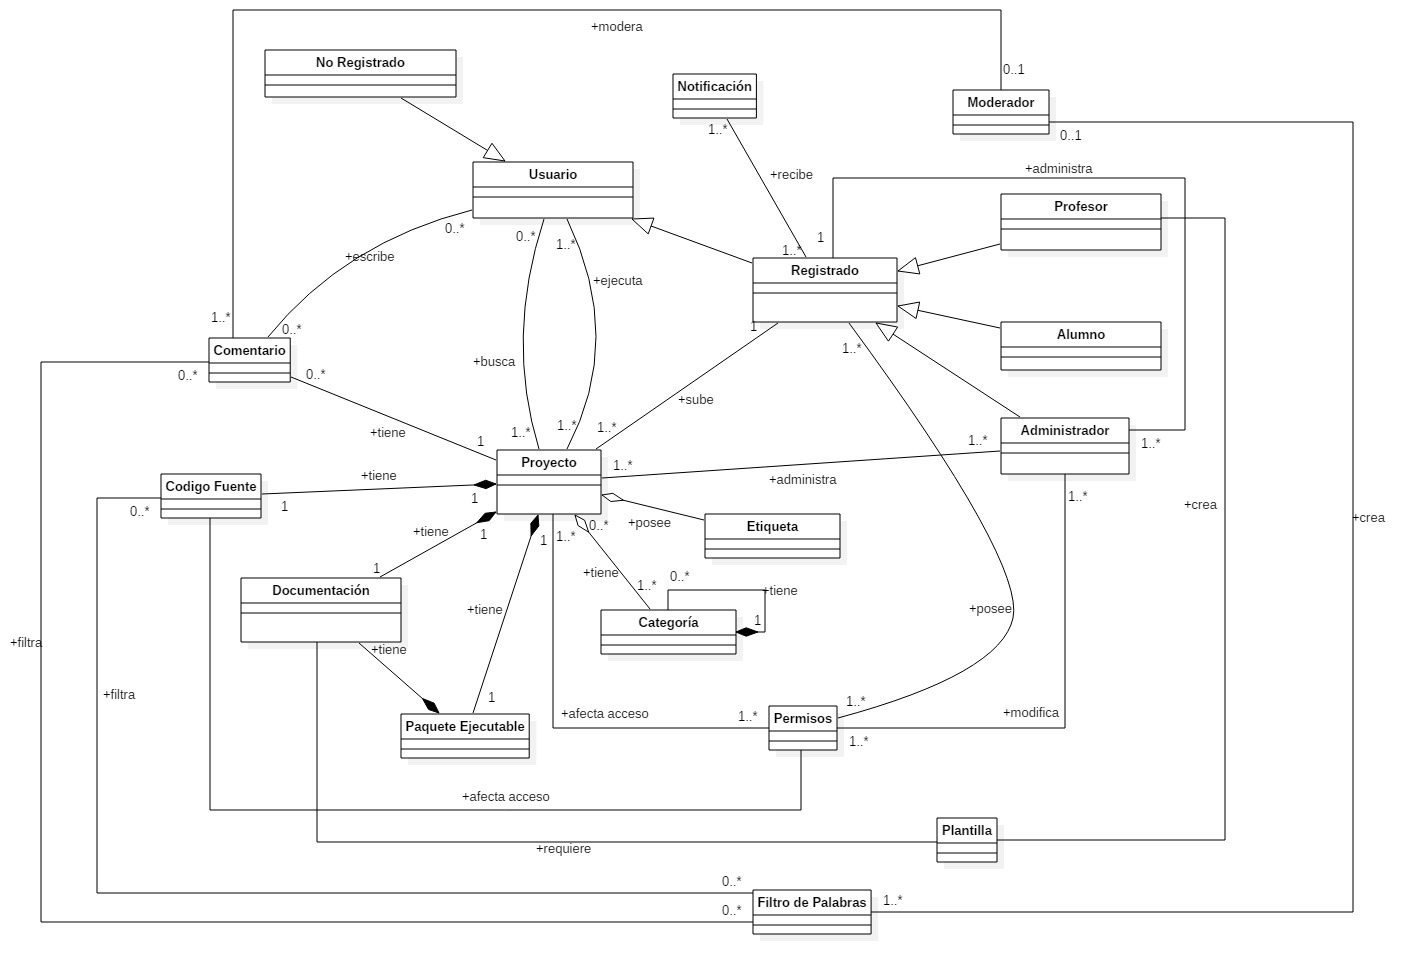
\includegraphics[width=\textwidth]{images/class/class}
\label{FIG:ER_DIA}
\caption{Diagrama de clases}
\end{figure}

\begin{figure}[!ht]
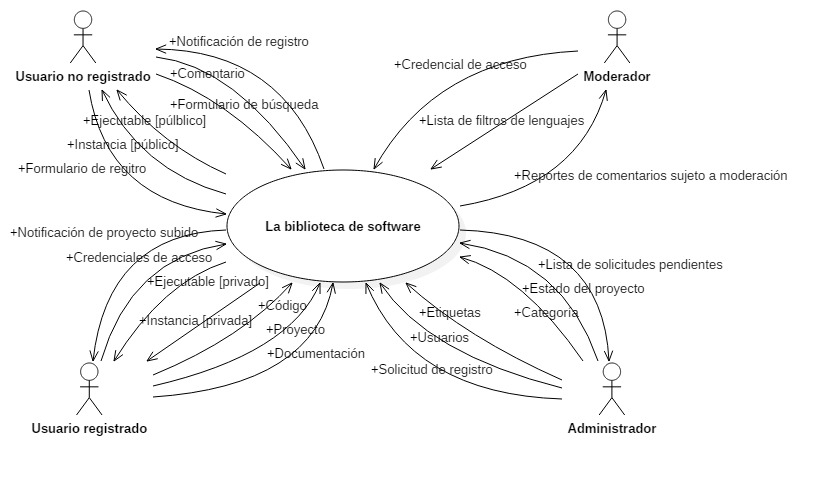
\includegraphics[width=\textwidth]{images/context/context0}
\label{FIG:ER_DIA}
\caption{Diagrama Diagrama de contexto nivel 0}
\end{figure}


\begin{figure}[!ht]
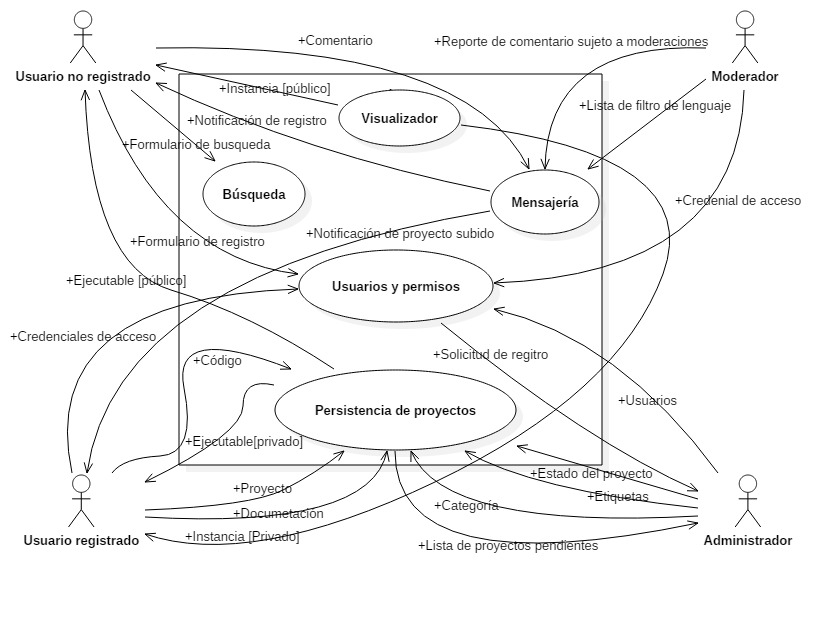
\includegraphics[width=\textwidth]{images/context/context1}
\label{FIG:ER_DIA}
\caption{Diagrama Diagrama de contexto nivel 1}
\end{figure}


\section{Divisi�n de tareas}
\section{Especificando un caso de uso en el negocio}

\section{Casos de uso de negocio}
\subsection{Lista y resumen de casos de uso de negocio}
\newpage
\section{Usuario}
\begin{table}[!ht]
\begin{tabular}{|c|p{2.5cm}|p{2.5cm}|p{2.5cm}|p{6cm}|}
\hline
	ID & Evento de Negocio & Input & Output & Summary \\ \hline
	BUC\_01 & Usuario se registra & Formulario de registro & - & Usuario llena el formulario de registro con la informaci�n necesaria (informaci�n b�sica y afiliaci�n). Luego el formulario le es enviado al administrador. \\ \hline
	BUC\_02 & Usuario comenta un proyecto & Formulario de comentario & - & Usuario ingresa su correo y nombre y deja un comentario. Este queda con visibilidad oculta hasta ser aprobado por un moderador. \\ \hline
	BUC\_03 & Usuario busca proyecto & Formulario de b�squeda & Lista de proyectos que empaten los criterios del formulario & Usuario ingresa los campos de b�squeda. Recibe una lista de proyectos con los proyectos m�s similes a sus criterios de b�squeda \\ \hline
	BUC\_04 & Usuario descarga proyecto (p�blico) & Identificador proyecto & Paquete descargable & Usuario selecciona descargar en un proyecto que est� revisando. En caso de estar disponible un paquete y ser parte de un proyecto p�blico, este se descarga. En caso contrario se indica que no est� disponible. \\ \hline
	BUC\_05 & Usuario solicita instancia de prueba para aplicaci�n (p�blica) (live) & Identificador proyecto & Instancia de prueba live & Usuario selecciona "prueba live" en un proyecto. En caso de estar disponible y de ser parte de un proyecto p�blico, este lanza una nueva ventana en el navegador con una instancia del proyecto en l�nea para su evaluaci�n por un periodo limitado de tiempo. \\ \hline
\end{tabular}
\end{table}

\newpage
\section{Usuario Registrado}
\begin{table}[!ht]
\begin{tabular}{|c|p{2.5cm}|p{2.5cm}|p{2.5cm}|p{6cm}|}
	\hline
	ID & Evento de Negocio & Input & Output & Summary \\ \hline
	BUC\_06 & Usuario (Registrado) descarga proyecto (privado) & Identificador proyecto & Paquete descargable & Usuario selecciona descargar en un proyecto que est� revisando. En caso de estar disponible un paquete, ser parte de un proyecto privado y si el usuario tiene los permisos necesarios para acceder a el, este se descarga. En caso contrario se indica que no est� disponible. \\ \hline
	BUC\_07 & Usuario (Registrado) crea proyecto & Descripci�n de proyecto &  & Usuario crea un nuevo proyecto indicando nombre, etiquetas y categor�as afectas. Este es almacenado con visibilidad oculta hasta que el usuario marque que est� enviado a revisi�n. \\ \hline
	BUC\_08 & Usuario (Registrado) sube codigo fuente & Identificador proyecto, Codigo fuente &  & Usuario completa formulario para agregar codigo fuente a un proyecto existente. \\ \hline
	BUC\_09 & Usuario (Registrado) sube documentacion & Identificador proyecto, Documentacion &  & Usuario completa formulario para agregar documentaci�n a un proyecto existente. \\ \hline
	BUC\_10 & Usuario (Registrado) sube ejecutables & Identificador proyecto, Ejecutable(s) &  & Usuario completa formulario para agregar ejecutables a un proyecto existente. \\ \hline
	BUC\_11 & Usuario (Registrado) envia proyecto a revisi�n & Identificador proyecto & Notificaci�n a administrador de nuevo env�o & Usuario env�a el proyecto a revisi�n. Todos los campos se congelan y el administrador es notificado que este proyecto est� listo para ser revisado. \\ \hline
	BUC\_12 & Usuario (Registrado) inicia sesi�n & Credenciales de acceso &  & Usuario llena el formulario de sesi�n con los datos requeridos (Nombre de Usuario y Contrase�a). En caso de que coincida con los datos persistentes inicia sesi�n. En caso contrario, notifica al usuario. \\ \hline
\end{tabular}
\end{table}

\newpage
\section{Moderador}
\begin{table}[!ht]
\begin{tabular}{|c|p{2.5cm}|p{2.5cm}|p{2.5cm}|p{6cm}|}
\hline
	ID & Evento de Negocio & Input & Output & Summary \\ \hline
 BUC\_13 & Moderador recibe comentario sujeto a moderaci�n &  & Comentario a revisar, Notificaci�n & De existir comentario pendiente recibe una notificaci�n y el comentario sujeto a moderaci�n. \\ \hline
	BUC\_14 & Moderador acepta o rechaza un comentario & Identificador de comentario, acci�n &  & Moderador elige un comentario. De cumplir con las normas establecidas, acepta el comentario. En caso contrario, lo rechaza \\ \hline
	BUC\_15 & Moderador agrega filtro de lenguaje & Especificaci�n de nuevo filtro de lenguaje
 &  & Moderador agrega nueva palabra a filtrar. De no existir, la persiste y notifica al moderador. En caso contrario, notifica al moderador. \\ \hline
	BUC\_16 & Moderador modifica filtro de lenguaje & Identificador de filtro de lenguaje, especificaci�n nueva de filtro de lenguaje &  & Moderador elige una palabra existente. De existir, la modifica y luego env�a los cambios. \\ \hline
	BUC\_17 & Moderador ingresa al sistema & Credenciales de acceso &  & Moderador llena el formulario de sesi�n con los datos requeridos (Nombre de Usuario y Contrase�a). En caso de que coincida con los datos persistentes inicia sesi�n. En caso contrario, notifica al moderador. \\ \hline
\end{tabular}
\end{table}

\newpage
\section{Administrador}
\begin{center}
\begin{table}[!ht]
\begin{tabular}{|c|p{2.8cm}|p{2.8cm}|p{2.5cm}|p{6cm}|}
\hline
	ID & Evento de Negocio & Input & Output & Summary \\ \hline
	BUC\_18 & Usuario (Administrador) recibe proyectos pendientes de moderacion &  & Lista de proyectos pendientes & Adminitrador revisa solicitudes de proyectos enviados para ser evaluados \\ \hline
	BUC\_19 & Usuario (Administrador) evalua proyecto pendiente & Identificador de proyecto, estado de visibilidad, comentario (opcional) & Notificacion a usuario afecto & Administrador revisa que los componentes del proyecto cumplan con las normas, segun esto procede a aceptar o rechazar la publicacion de un proyecto y genera una notificacion al usuario encargado del proyecto \\ \hline
	BUC\_20 & Usuario (Administrador) recibe solicitudes de cuentas pendientes &  & Lista de solicitudes de cuentas & Adminitrador revisa solicitudes de cuentas enviados por usuarios no registrados para crear una nueva cuenta \\ \hline
	BUC\_21 & Usuario (Administrador) agrega una etiqueta &  & Etiqueta nueva & Administrador agrega una etiqueta. De no existir, crea la etiqueta. En caso contrario, notifica al moderador. \\ \hline
	BUC\_22 & Usuario (Administrador) agrega una categor�a &  & Categor�a nueva & Administrador agrega una categor�a. De no existir, crea la categor�a. En caso contrario, notifica al Administrador \\ \hline
	BUC\_23 & Usuario (Administrador) modifica una etiqueta & Identificador de etiqueta, especificaci�n nueva de etiqueta &  & Administrador elige una etiqueta. De existir, modifica la etiqueta y env�a los cambios. \\ \hline
	BUC\_24 & Usuario (Administrador) modifica una categor�a & Identificador de categor�a, especificaci�n nueva de categor�a &  & Administrador elige una categor�a. De existir, modifica la categor�a y env�a los cambios. \\ \hline
\end{tabular}
\end{table}
\end{center}
\newpage
\begin{center}
\begin{table}[!ht]
\begin{tabular}{|c|p{2.8cm}|p{2.8cm}|p{2.5cm}|p{6cm}|}
\hline
	ID & Evento de Negocio & Input & Output & Summary \\ \hline
	BUC\_25 & Usuario (Administrador) modifica visibilidad de proyecto & Identificador de proyecto, estado de visibilidad & Notificacion al usuario afectado & Administrador selecciona un proyecto y cambia su visibilidad. Luego, se le env�a una notificaci�n al usuario afectado. \\ \hline
	BUC\_26 & Usuario (Administrador) modifica cuenta & Identificador de cuenta, especificaci�n nueva de cuenta & Notificacion al usuario afectado & Administrador elige cuenta de usuario. De existir, el administrador modifica la cuenta y env�a los cambios. \\ \hline
	BUC\_27 & Usuario (Administrador) configura instanciado de proyecto & Configuracion especifica para el proyecto &  & Administrador configura el visualizador segun los requisitos de funcionamiento del proyecto \\ \hline
	BUC\_28 & Borrar categoria & Categoria &  & Administrador selecciona la categoria y la elimina \\ \hline
	BUC\_29 & Borrar etiqueta & Etiqueta &  & Administrador selecciona la etiqueta y la elimina \\ \hline
	BUC\_30 & Usuario (Administrador) modifica proyecto en espera de aceptacion & Identificador de proyecto, modificaciones & Notificacion al usuario & Administrador cambia o quita componentes del proyecto que no cumplan con las normas, luego de esto se envia una notificacion al usuario de la modificacion \\ \hline
\end{tabular}
\end{table}
\end{center}
\subsection{Casos de uso de negocio}

\begin{table}[]
\centering
\caption{BUC_01}
\resizebox{\textwidth}{!}{%
\begin{tabular}{|p{3cm}|p{7cm}|}
\hline
\textbf{Business Event} & Usuario decide registrarse                                                                                                    \\ \hline
\textbf{BUC Name}       & Usuario se registra                                                                                                           \\ \hline
\textbf{Triggers}       & Administrador existente                                                                                                       \\ \hline
\textbf{Precondiciones}  & Ninguno                                                                                                                       \\ \hline
\textbf{SH Interesados}  & Usuarios no registrados, Administradores, subsistemas de Usuarios y permisos, subsistema de Mensajer�a.                       \\ \hline
\textbf{SH Activos}      & Usuarios no registrados, Administradores.                                                                                     \\ \hline
\multicolumn{2}{|l|}{\textbf{Escenario}}                                                                                                                \\ \hline
1.-            & Abrir el formulario de registro.                                                                                              \\ \hline
2.-            & Ingresar el nombre de usuario.                                                                                                \\ \hline
3.-            & Ingresar el correo electr�nico.                                                                                               \\ \hline
E3.1           & Correo electr�nico ya existente.                                                                                              \\ \hline
4.-            & Ingresar la contrase�a.                                                                                                       \\ \hline
5.-            & Enviar el registro.                                                                                                           \\ \hline
A4.1           & Cancelar el registro.                                                                                                         \\ \hline
6.-            & El Administrador recibe una notificaci�n con una solicitud de registro pendiente.                                             \\ \hline
\textbf{Outcome}        & El usuario env�a el registro de usuario al administrador. El administrador recibe una notificaci�n con un registro pendiente. \\ \hline
\end{tabular}%
}
\end{table}

\begin{figure}[!ht]
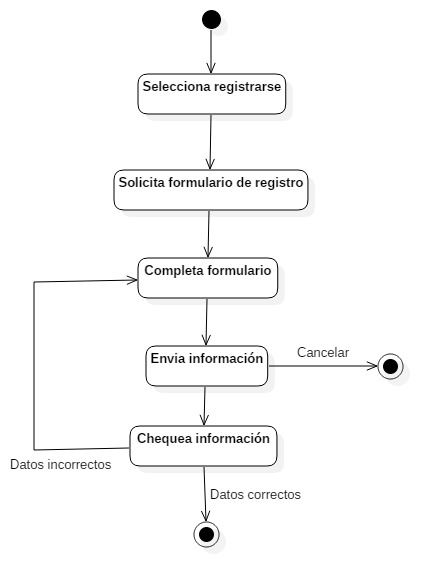
\includegraphics[width=\textwidth]{images/sec/1.jpg}
\label{FIG:CU_PUC01}
\caption{Diagrama de secuencia de uso para BUC_01: Registrar usuario}
\end{figure}


\begin{table}[]
\centering
\caption{BUC_02}
\resizebox{\textwidth}{!}{%
\begin{tabular}{|p{3cm}|p{7cm}|}
\hline
\textbf{Business Event} & Usuario decide realizar un comentario sobre un proyecto                                                                                   \\ \hline
\textbf{BUC Name}       & Usuario comenta un proyecto                                                                                                               \\ \hline
\textbf{Triggers}       & Proyecto existente, comentario                                                                                                            \\ \hline
\textbf{Precondiciones}  & El usuario debe tener el nivel de acceso requerido acceder al proyecto                                                                    \\ \hline
\textbf{SH Interesados}  & Usuarios registrados, Usuarios no registrados, Moderadores, mensajer�a, persistencia de proyectos                                         \\ \hline
\textbf{SH Activos}      & Usuarios registrados                                                                                                                      \\ \hline
\multicolumn{2}{|l|}{\textbf{Escenario}}                                                                                                                            \\ \hline
1.-            & Encontrar un proyecto en la plataforma                                                                                                    \\ \hline
2.-            & Redactar un comentario                                                                                                                    \\ \hline
3.-            & Enviar el comentario o bien cancelar la operaci�n                                                                                         \\ \hline
A3.1           & Cancelar el env�o del comentario                                                                                                          \\ \hline
4.-            & Indicar al usuario que el comentario fue recibido y est� pendiente de aceptaci�n por parte del moderador.                                 \\ \hline
\textbf{Outcome}        & El usuario envia un comentario a moderaci�n, el moderador recibe una notificaci�n de que hay un nuevo comentario pendiente de moderaci�n. \\ \hline
\end{tabular}%
}
\end{table}

\begin{table}[]
\centering
\caption{BUC_03}
\resizebox{\textwidth}{!}{%
\begin{tabular}{|p{3cm}|p{7cm}|}
\hline
\textbf{Business Event} & Usuario busca un proyecto dentro de la plataforma                                                                            \\ \hline
\textbf{BUC Name}       & Usuario busca proyecto                                                                                                       \\ \hline
\textbf{Triggers}       & Usuario, par�metros de b�squeda                                                                                              \\ \hline
\textbf{Precondiciones}  & Niguno                                                                                                                       \\ \hline
\textbf{SH Interesados}  & Usuarios de cualquier tipo, busqueda de proyectos, persistencia de proyectos                                                 \\ \hline
\textbf{SH Activos}      & Usuarios de cualquier tipo                                                                                                   \\ \hline
\multicolumn{2}{|l|}{\textbf{Escenario}}                                                                                                               \\ \hline
1.-            & Ingresar al m�dulo de b�squeda                                                                                               \\ \hline
2.-            & Ingresar categor�as a buscar                                                                                                 \\ \hline
A2.1.          & No se seleccionan categor�as                                                                                                 \\ \hline
3.-            & Ingresar etiquetas a buscar                                                                                                  \\ \hline
A3.1.          & No se seleccionan etiquetas                                                                                                  \\ \hline
4.-            & Ingresar palabras clave de la descripci�n o t�tulo                                                                           \\ \hline
A3.1.          & No se seleccionan palabras clave                                                                                             \\ \hline
5.-            & Ejecutar b�squeda                                                                                                            \\ \hline
\textbf{Outcome}        & El usuario recibe una lista con los proyectos que encajan con los criterios de b�squeda proporcionados y su nivel de acceso. \\ \hline
\end{tabular}%
}
\end{table}

\begin{table}[]
\centering
\caption{BUC_04}
\resizebox{\textwidth}{!}{%
\begin{tabular}{|p{3cm}|p{7cm}|}
\hline
\textbf{Business Event} & Usuario decide descargar proyecto p�blico.                                                                           \\ \hline
\textbf{BUC Name}       & Usuario descarga proyecto (P�blico)                                                                                  \\ \hline
\textbf{Triggers}       & Usuario, proyecto p�blico existente.                                                                                 \\ \hline
\textbf{Precondiciones}  & BUC\_03 (Usuario busca proyecto)                                                                                     \\ \hline
\textbf{SH Interesados}  & Usuarios Registrados, Usuarios no Registrados, Subsistema Usuarios y Permisos, Subsistema Persistencia de Proyectos. \\ \hline
\textbf{SH Activos}      & Usuarios registrados, Usuarios no registrados.                                                                       \\ \hline
\multicolumn{2}{|l|}{\textbf{Escenario}}                                                                                                       \\ \hline
1.-            & Encontrar un proyecto en la plataforma.                                                                              \\ \hline
2.-            & Descargar un proyecto.                                                                                               \\ \hline
A2.1           & El usuario recibir� una notificaci�n de que el proyecto no se encuentra disponible.                                  \\ \hline
A2.2           & Descarga cancelada.                                                                                                  \\ \hline
\textbf{Outcome}        & El usuario recibe un paquete con los archivos correspondientes al proyecto.                                          \\ \hline
\end{tabular}%
}
\end{table}


% Please add the following required packages to your document preamble:
% \usepackage{graphicx}
\begin{table}[]
\centering
\caption{BUC_05}
\resizebox{\textwidth}{!}{%
\begin{tabular}{|p{3cm}|p{7cm}|}
\hline
\textbf{Business Event} & Usuario busca un proyecto dentro de la plataforma                            \\ \hline
\textbf{BUC Name}       & Usuario solicita instancia de prueba para aplicaci�n (p�blica) (live)        \\ \hline
\textbf{Triggers}       & Usuario, par�metros de b�squeda                                              \\ \hline
\textbf{Precondiciones}  & El usuario debe tener el nivel de acceso requerido acceder al proyecto       \\ \hline
\textbf{SH Interesados}  & Usuarios de cualquier tipo, busqueda de proyectos, persistencia de proyectos \\ \hline
\textbf{SH Activos}      & Usuarios de cualquier tipo                                                   \\ \hline
\multicolumn{2}{|l|}{\textbf{Escenario}}                                                               \\ \hline
1.-            & Encontrar un proyecto en la plataforma                                       \\ \hline
2.-            & Seleccionar opci�n ``Live ''test"                                               \\ \hline
E2.1           & Opcion de ``Live test'' no disponible                                          \\ \hline
3.-            & Ingresar al enlace provisto                                                  \\ \hline
E3.1           & Instanciaci�n de prueba falla                                                \\ \hline
\textbf{Outcome}        & El usuario es redirigido a un sitio que muestra el proyecto ejecut�ndose     \\ \hline
\end{tabular}%
}
\end{table}


% Please add the following required packages to your document preamble:
% \usepackage{graphicx}
\begin{table}[]
\centering
\caption{BUC_06}
\resizebox{\textwidth}{!}{%
\begin{tabular}{|p{3cm}|p{7cm}|}
\hline
\textbf{Business Event} & Usuario registrado decide descargar proyecto privado                                        \\ \hline
\textbf{BUC Name}       & Usuario (Registrado) descarga proyecto (privado)                                            \\ \hline
\textbf{Triggers}       & Usuario Registrado, proyecto privado existente.                                             \\ \hline
\textbf{Precondiciones}  & El usuario debe tener el nivel de acceso requerido para acceder al proyecto.                \\ \hline
\textbf{SH Interesados}  & Usuarios Registrados, Subsistema Usuarios y Permisos, Subsistema Persistencia de Proyectos. \\ \hline
\textbf{SH Activos}      & Usuarios Registrados.                                                                       \\ \hline
\multicolumn{2}{|l|}{\textbf{Escenario}}                                                                              \\ \hline
1.-            & Encontrar un proyecto en la plataforma.                                                     \\ \hline
2.-            & Descargar un proyecto.                                                                      \\ \hline
A2.1           & El usuario recibir� una notificaci�n de que el proyecto no se encuentra disponible.         \\ \hline
A2.2           & Descarga cancelada.                                                                         \\ \hline
\textbf{Outcome}        & El usuario recibe un paquete con los archivos correspondientes al proyecto.                 \\ \hline
\end{tabular}%
}
\end{table}

% Please add the following required packages to your document preamble:
% \usepackage{graphicx}
\begin{table}[]
\centering
\caption{BUC_07}
\resizebox{\textwidth}{!}{%
\begin{tabular}{|p{3cm}|p{7cm}|}
\hline
\textbf{Business Event} & Usuario registrado decide crear proyecto                                                                                                               \\ \hline
\textbf{BUC Name}       & Usuario (Registrado) crea proyecto                                                                                                                     \\ \hline
\textbf{Triggers}       & Usuarios registrados                                                                                                                                   \\ \hline
\textbf{Precondiciones}  & El usuario debe tener el nivel de acceso requerido para acceder al proyecto                                                                            \\ \hline
\textbf{SH Interesados}  & Usuarios registrados, Usuarios no registrados, Administradores, Subsistema de mensajer�a, Subsistema de Proyectos y persistencia                       \\ \hline
\textbf{SH Activos}      & Usuarios registrados, Administradores, Moderadores                                                                                                     \\ \hline
\multicolumn{2}{|l|}{\textbf{Escenario}}                                                                                                                                         \\ \hline
1.-            & Ingresar al m�dulo de crear proyectos                                                                                                                  \\ \hline
2.-            & Ingresar el nombre del proyecto                                                                                                                        \\ \hline
3.-            & Ingresar la descripci�n del proyecto                                                                                                                   \\ \hline
4.-            & Ingresar el autor                                                                                                                                      \\ \hline
5.-            & Ingresar la fecha de creaci�n                                                                                                                          \\ \hline
6.-            & Ingresar el correo electr�nico                                                                                                                         \\ \hline
7.-            & Ingresar el curso de origen                                                                                                                            \\ \hline
8.-            & Ingresar especificaciones (sistema operativo, leguaje, prerequisitos, sobre instalacion),                                                              \\ \hline
9.-            & Seleccionar y agregar etiquetas                                                                                                                        \\ \hline
E.9            & Etiqueta se encuentra asignada al proyecto                                                                                                             \\ \hline
10.-           & Seleccionar y agregar categor�as                                                                                                                       \\ \hline
E.10           & Categoria se encuentra asignada al proyecto                                                                                                            \\ \hline
11.-           & Seleccionar visivilidad del proyecto                                                                                                                   \\ \hline
12.-           & Crear proyecto                                                                                                                                         \\ \hline
A.12.1         & Cancelar crear proyecto                                                                                                                                \\ \hline
\textbf{Outcome}        & Usuario almacena la informaci�n del proyecto a crear. Al momento de guardar la informacion se visualiza una notificaci�n de perfil de proyecto creado. \\ \hline
\end{tabular}%
}
\end{table}

% Please add the following required packages to your document preamble:
% \usepackage{graphicx}
\begin{table}[]
\centering
\caption{BUC_08}
\resizebox{\textwidth}{!}{%
\begin{tabular}{|p{3cm}|p{7cm}|}
\hline
\textbf{Business Event} & Usuario registrado decide subir el c�digo fuente                                      \\ \hline
\textbf{BUC Name}       & Usuario Registrado sube codigo fuente                                                 \\ \hline
\textbf{Triggers}       & Usuario Registrado, proyecto privado existente.                                       \\ \hline
\textbf{Precondiciones}  & Perfil de proyecto creado, usuario identificado                                       \\ \hline
\textbf{SH Interesados}  & Usuarios Registrados, Subsistema Usuarios y Permisos                                  \\ \hline
\textbf{SH Activos}      & Usuarios Registrados.                                                                 \\ \hline
\multicolumn{2}{|l|}{\textbf{Escenario}}                                                                        \\ \hline
1.             & Ingresar al perfil del proyecto                                                       \\ \hline
2.             & Seleccionar subir c�digo fuente                                                       \\ \hline
3.             & Subir c�digo fuente.                                                                  \\ \hline
E.3.1          & El C�digo fuente ya fue subido.                                                       \\ \hline
A.3.1          & Cancelar Operaci�n                                                                    \\ \hline
\textbf{Outcome}        & El usuario sube un c�digo fuente que se encuentra asciado a un perfil de un proyecto. \\ \hline
\end{tabular}%
}
\end{table}

% Please add the following required packages to your document preamble:
% \usepackage{graphicx}
\begin{table}[]
\centering
\caption{BUC_09}
\resizebox{\textwidth}{!}{%
\begin{tabular}{|p{3cm}|p{7cm}|}
\hline
\textbf{Business Event} & Usuario desea subir documentacion             \\ \hline
\textbf{BUC Name}       & Subir documentacion                           \\ \hline
\textbf{Triggers}       & Usuario                                       \\ \hline
\textbf{Precondiciones}  & Proyecto seleccionado o En subida de proyecto \\ \hline
\textbf{SH Interesados}  & Usuario                                       \\ \hline
\textbf{SH Activos}      & Usuario                                       \\ \hline
\multicolumn{2}{|l|}{\textbf{Escenario}}                                \\ \hline
1              & Seleccionar documentacion                     \\ \hline
E1.1           & La documentacion no cumple con las normas     \\ \hline
E1.2           & No se pudo cargar la documentacion            \\ \hline
A1.3           & Cancelar la operacion                         \\ \hline
2              & Enviar documentacion                          \\ \hline
\textbf{Outcome}        & Documentacion de un proyecto entregada        \\ \hline
\end{tabular}%
}
\end{table}

% Please add the following required packages to your document preamble:
% \usepackage{graphicx}
\begin{table}[]
\centering
\caption{BUC_10}
\resizebox{\textwidth}{!}{%
\begin{tabular}{|p{3cm}|p{7cm}|}
\hline
\textbf{Business Event} & Usuario desea subir ejecutables               \\ \hline
\textbf{BUC Name}       & Subir ejecutables                             \\ \hline
\textbf{Triggers}       & Usuario                                       \\ \hline
\textbf{Precondiciones}  & Proyecto seleccionado o En subida de proyecto \\ \hline
\textbf{SH Interesados}  & Usuarios Registrados                          \\ \hline
\textbf{SH Activos}      & Usuarios Registrados                          \\ \hline
\multicolumn{2}{|l|}{\textbf{Escenario}}                                \\ \hline
1              & Seleccionar ejecutable                        \\ \hline
E1.1           & El ejecutable fuente no cumple con las normas \\ \hline
E1.2           & No se pudo cargar el ejecutable               \\ \hline
A1.3           & Cancelar la operacion                         \\ \hline
2              & Enviar ejecutable                             \\ \hline
\textbf{Outcome}        & Ejecutable de un proyecto disponible en el.   \\ \hline
\end{tabular}%
}
\end{table}

% Please add the following required packages to your document preamble:
% \usepackage{graphicx}
\begin{table}[]
\centering
\caption{BUC_11}
\resizebox{\textwidth}{!}{%
\begin{tabular}{|p{3cm}|p{7cm}|}
\hline
\textbf{Business Event} & Usuario registrado decide enviar proyecto a revision                                                                                                                                                         \\ \hline
\textbf{BUC Name}       & Usuario (Registrado) envia proyecto a revisi�n                                                                                                                                                               \\ \hline
\textbf{Triggers}       & Usuarios registrados                                                                                                                                                                                         \\ \hline
\textbf{Precondiciones}  & El usuario debe tener el nivel de acceso requerido para acceder al proyecto                                                                                                                                  \\ \hline
\textbf{SH Interesados}  & Usuarios registrados, Usuarios no registrados, Administradores, Subsistema de mensajer�a, Subsistema de Proyectos y persistencia                                                                             \\ \hline
\textbf{SH Activos}      & Usuarios registrados, Administradores, Moderadores                                                                                                                                                           \\ \hline
\multicolumn{2}{|l|}{\textbf{Escenario}}                                                                                                                                                                                               \\ \hline
1.-            & Ingresar al m�dulo de proyectos creados                                                                                                                                                                      \\ \hline
2.-            & Seleccionar el proyecto a enviar                                                                                                                                                                             \\ \hline
E.2.1          & El C�digo fuente no se encuentra.                                                                                                                                                                            \\ \hline
               & La documentacion del proyecto no se ecuentra                                                                                                                                                                 \\ \hline
               & El ejecutable del proyecto no se encuentra                                                                                                                                                                   \\ \hline
A.3.1          & Cancelar Operaci�n                                                                                                                                                                                           \\ \hline
4.-            & Cambiar estado de visibilidad a enviado a revision                                                                                                                                                           \\ \hline
5.-            & Guardar cambios                                                                                                                                                                                              \\ \hline
A.5.1          & Cancelar Operaci�n                                                                                                                                                                                           \\ \hline
\textbf{Outcome}        & Usuario envia proyecto a evaluacion. Recibe una notificaci�n de que el proyecto ha sido enviado mientras que el administrador y el moderador son notificados que este proyecto est� listo para ser revisado. \\ \hline
\end{tabular}%
}
\end{table}

% Please add the following required packages to your document preamble:
% \usepackage{graphicx}
\begin{table}[]
\centering
\caption{BUC_12}
\resizebox{\textwidth}{!}{%
\begin{tabular}{|p{3cm}|p{7cm}|}
\hline
\textbf{Business Event} & Usuario registrado decide iniciar sesion                                                               \\ \hline
\textbf{BUC Name}       & Usuario Registrado inicia sesi�n                                                                       \\ \hline
\textbf{Triggers}       & Usuario Registrado                                                                                     \\ \hline
\textbf{Precondiciones}  & El usuario debe tener una cuenta creada en la plataforma.                                              \\ \hline
\textbf{SH Interesados}  & Usuarios Registrados, Subsistema Usuarios y Permisos                                                   \\ \hline
\textbf{SH Activos}      & Usuarios Registrados.                                                                                  \\ \hline
\multicolumn{2}{|l|}{\textbf{Escenario}}                                                                                         \\ \hline
1.             & Ingresar al m�dulo de inicio de sesi�n                                                                 \\ \hline
2.             & Ingresar nombre de usuario                                                                             \\ \hline
3.             & Ingresar contrase�a                                                                                    \\ \hline
4.             & Iniciar sesi�n.                                                                                        \\ \hline
A4.1           & Env�a una notificaci�n al usuarios acerca de sus datos que no coincidieron con los datos persistentes. \\ \hline
A4.2           & Operaci�n Cancelada.                                                                                   \\ \hline
\textbf{Outcome}        & El usuario inicia sesion y es redirigido a la p�gina principal.                                        \\ \hline
\end{tabular}%
}
\end{table}

\begin{table}[]
\centering
\caption{BUC_13}
\resizebox{\textwidth}{!}{%
\begin{tabular}{|p{3cm}|p{7cm}|}
\hline
\textbf{Business Event} & El moderador recibe un comentario sujeto a moderaci�n.                                                         \\ \hline
\textbf{BUC Name}       & Moderador recibe comentario sujeto a moderaci�n                                                                \\ \hline
\textbf{Triggers}       & Usuario Registrado                                                                                             \\ \hline
\textbf{Precondiciones}  & El moderador debe tener el nivel de acceso requerido para recibir la notificaci�n. Debe existir un comentario. \\ \hline
\textbf{SH Interesados}  & Moderadores, Usuarios Registrados, Subsistema Usuarios y Permisos, Subsistema Mensajer�a, Administrador        \\ \hline
Active SH      & Moderadores, Administrador                                                                                     \\ \hline
\multicolumn{2}{|l|}{\textbf{\textbf{Escenario}}}                                                                                                 \\ \hline
1.             & Recibir una notificaci�n de un nuevo comentario.                                                               \\ \hline
2.             & Ingresar al m�dulo de moderaci�n de comentarios.                                                               \\ \hline
3.             & Recibir un nuevo comentario.                                                                                   \\ \hline
E3.1           & No existe ning�n comentario recibido.                                                                          \\ \hline
A3.1           & Operaci�n Cancelada.                                                                                           \\ \hline
\textbf{Outcome}        & El moderador recibe un comentario sujeto a moderaci�n.                                                         \\ \hline
\end{tabular}%
}
\end{table}

% Please add the following required packages to your document preamble:
% \usepackage{graphicx}
\begin{table}[]
\centering
\caption{BUC_14}
\resizebox{\textwidth}{!}{%
\begin{tabular}{|p{3cm}|p{7cm}|}
\hline
\textbf{Business Event} & El Moderador decide aceptar o rechazar un comentario                                                                   \\ \hline
\textbf{BUC Name}       & Moderador acepta o rechaza un comentario                                                                               \\ \hline
\textbf{Triggers}       & Moderador                                                                                                              \\ \hline
\textbf{Precondiciones} & El moderador debe tener el nivel de acceso requerido para poder realizar la operaci�n. Debe existir un comentario.     \\ \hline
\textbf{SH Interesados} & Moderadores, Usuarios Registrados, Subsistema Usuarios y Permisos, Subsistema Mensajer�a, Administrador                \\ \hline
Active SH                 & Usuarios Registrados, Moderadores o Administrador                                                                      \\ \hline
\multicolumn{2}{|l|}{\textbf{Escenario}}                                                                                                                    \\ \hline
1.                        & Ingresar al m�dulo de moderaci�n de comentarios.                                                                       \\ \hline
2.                        & Abrir un nuevo comentario a moderar.                                                                                   \\ \hline
E2.1                      & No existe ning�n comentario recibido.                                                                                  \\ \hline
3.                        & Revisar comentario.                                                                                                    \\ \hline
4.                        & Aceptar Comentario.                                                                                                    \\ \hline
A4.1                      & Rechazar Comentario.                                                                                                   \\ \hline
A4.2                      & Operaci�n Cancelada.                                                                                                   \\ \hline
5.                        & Env�a al usuario una notificaci�n de comentario aceptado.                                                              \\ \hline
E5.1                      & Env�a al usuario una notificaci�n de comentario rechazado.                                                             \\ \hline
\textbf{Outcome}        & El usuario recibe una notificaci�n de comentario aceptado. El comentario es mostrado en el proyecto donde se escribi�. \\ \hline
\end{tabular}%
}
\end{table}

\begin{table}[]
\centering
\caption{BUC_15}
\resizebox{\textwidth}{!}{%
\begin{tabular}{|p{3cm}|p{7cm}|}
\hline
\textbf{Business Event} & Moderador agrega filtro de lenguaje             \\ \hline
\textbf{BUC Name}       & Agregar filtro de lenguaje                      \\ \hline
\textbf{Triggers}       & Moderador                                       \\ \hline
\textbf{Precondiciones}  & Moderador identificado                          \\ \hline
\textbf{SH Interesados}  & Moderador, Administrador                        \\ \hline
Active SH      & Moderador, Administrador                        \\ \hline
\multicolumn{2}{|l|}{\textbf{\textbf{Escenario}}}                                  \\ \hline
1              & Solicitar ingreso de nuevo filtro               \\ \hline
2              & Ingresar nueva palabra a filtrar                \\ \hline
3              & Enviar el nuevo filtro                          \\ \hline
E3.1           & La palabra ingresada ya existe                  \\ \hline
\textbf{Outcome}        & Nueva palabra en la lista de filtro de palabras \\ \hline
\end{tabular}%
}
\end{table}
\clearpage
\begin{table}[]
\centering
\caption{BUC_16}
\resizebox{\textwidth}{!}{%
\begin{tabular}{|p{3cm}|p{7cm}|}
\hline
\textbf{Business Event} & Moderador modifica filtro de lenguaje                    \\ \hline
\textbf{BUC Name}       & Modificar filtro de lenguaje                             \\ \hline
\textbf{Triggers}       & Moderador                                                \\ \hline
\textbf{Precondiciones}  & Moderador identificado. Moderador en la lista de filtros \\ \hline
\textbf{SH Interesados}  & Moderador, Administrador                                 \\ \hline
Active SH      & Moderador o Administrador                                \\ \hline
\multicolumn{2}{|l|}{\textbf{\textbf{Escenario}}}                                           \\ \hline
1              & Seleccionar filtro a modificar                           \\ \hline
2              & Modificar el filtro                                      \\ \hline
3              & Enviar la modificacion del filtro                        \\ \hline
E3.1           & La modificacion coincide con un filtro existente         \\ \hline
E3.2           & No se ha podido realizar la modificacion                 \\ \hline
\textbf{Outcome}        & Palabra seleccionada con modificacion realizada          \\ \hline
\end{tabular}%
}
\end{table}

\begin{table}[]
\centering
\caption{BUC_17}
\resizebox{\textwidth}{!}{%
\begin{tabular}{|p{3cm}|p{7cm}|}
\hline
\textbf{Business Event} & Moderador ingresa el sistema                                                                           \\ \hline
\textbf{BUC Name}       & Ingreso al sistema                                                                                     \\ \hline
\textbf{Triggers}       & Moderador                                                                                              \\ \hline
\textbf{Precondiciones}  & Moderador con cuenta en el sistema                                                                     \\ \hline
\textbf{SH Interesados}  & Moderador, Administrador                                                                               \\ \hline
Active SH      & Moderador o Administrador                                                                              \\ \hline
\multicolumn{2}{|l|}{\textbf{\textbf{Escenario}}}                                                                                         \\ \hline
1.             & Ingresar al m�dulo de inicio de sesi�n                                                                 \\ \hline
2.             & Ingresar nombre de usuario                                                                             \\ \hline
3.             & Ingresar contrase�a                                                                                    \\ \hline
4.             & Iniciar sesi�n.                                                                                        \\ \hline
A4.1           & Env�a una notificaci�n al usuarios acerca de sus datos que no coincidieron con los datos persistentes. \\ \hline
A4.2           & Operaci�n Cancelada.                                                                                   \\ \hline
\textbf{Outcome}        & Usuario identificado en el sistema como moderador                                                      \\ \hline
\end{tabular}%
}
\end{table}
\clearpage
\begin{table}[]
\centering
\caption{BUC_18}
\resizebox{\textwidth}{!}{%
\begin{tabular}{|p{3cm}|p{7cm}|}
\hline
\textbf{Business Event} & Administrador recibe lista de proyectos                         \\ \hline
\textbf{BUC Name}       & Revision lista de proyectos pendientes                          \\ \hline
\textbf{Triggers}       & Administrador, proyecto a ser administrado                      \\ \hline
\textbf{Precondiciones}  & Administrador identificado, proyecto en espera de moderacion    \\ \hline
\textbf{SH Interesados}  & Usuario, Administrador                                          \\ \hline
Active SH      & Administrador                                                   \\ \hline
\multicolumn{2}{|l|}{\textbf{\textbf{Escenario}}}                                                  \\ \hline
1.             & Ingresar a proyectos en espera de evaluacion                    \\ \hline
E1.1           & No hay proyectos en espera                                      \\ \hline
2              & Seleccionar un proyecto de la lista                             \\ \hline
E2.1           & Salir                                                           \\ \hline
\textbf{Outcome}        & El usuario inicia sesion y es redirigido a la p�gina principal. \\ \hline
\end{tabular}%
}
\end{table}

\begin{table}[]
\centering
\caption{BUC_19}
\resizebox{\textwidth}{!}{%
\begin{tabular}{|p{3cm}|p{7cm}|}
\hline
\textbf{Business Event} & Administrador evalua proyecto                   \\ \hline
\textbf{BUC Name}       & Evaluacion de proyectos                         \\ \hline
\textbf{Triggers}       & Administrador, proyecto.                        \\ \hline
\textbf{Precondiciones}  & Administrador, proyecto en espera de evaluacion \\ \hline
\textbf{SH Interesados}  & Usuario, Administrador                          \\ \hline
Active SH      & Administrador                                   \\ \hline
\multicolumn{2}{|l|}{\textbf{Escenario}}                                  \\ \hline
1.             & Descargar componentes del proyecto              \\ \hline
2              & Revisar informacion del proyecto                \\ \hline
3              & Revisar codigo fuente                           \\ \hline
4              & Revisar ejecutable                              \\ \hline
5              & Revisar documentacion                           \\ \hline
6              & Aceptar proyecto                                \\ \hline
A6.1           & Rechazar proyecto                               \\ \hline
7              & Generar notificacion al ``due�o'' del proyecto    \\ \hline
\textbf{Outcome}        & Proyecto publicado, notificacion generada       \\ \hline
\end{tabular}%
}
\end{table}

\begin{table}[]
\centering
\caption{BUC_20}
\resizebox{\textwidth}{!}{%
\begin{tabular}{|p{3cm}|p{7cm}|}
\hline
\textbf{Business Event} & Administrador evalua solicitudes de registro de cuenta                         \\ \hline
\textbf{BUC Name}       & Evaluacion de solicitudes de registro de cuenta                                \\ \hline
\textbf{Triggers}       & Administrador, solicitud de registro                                           \\ \hline
\textbf{Precondiciones}  & Administrador identificado, solicitud de registro elevada                      \\ \hline
\textbf{SH Interesados}  & Usuario no registrado                                                          \\ \hline
Active SH      & Administrador                                                                  \\ \hline
\multicolumn{2}{|l|}{\textbf{\textbf{Escenario}}}                                                                 \\ \hline
1.             & Seleccionar mostrar la lista de solicitudes pendientes                         \\ \hline
2              & Seleccionar una solicitud                                                      \\ \hline
3              & Revisar solicitud                                                              \\ \hline
4              & Aceptar solicitud                                                              \\ \hline
A4.1           & Rechazar solicitud                                                             \\ \hline
5              & Generar una notificacion al realizador de la solicitud                         \\ \hline
\textbf{Outcome}        & Solicitud aceptada, nueva cuenta generada, notificacion enviada al solicitador \\ \hline
\end{tabular}%
}
\end{table}

\begin{table}[]
\centering
\caption{BUC_21}
\resizebox{\textwidth}{!}{%
\begin{tabular}{|p{3cm}|p{7cm}|}
\hline
\textbf{Business Event} & Usuario Administrador decide agregar una etiqueta al proyecto en revisi�n                                                                                   \\ \hline
\textbf{BUC Name}       & Usuario (Administrador) agrega una etiqueta                                                                                                                 \\ \hline
\textbf{Triggers}       & Usuarios registrados                                                                                                                                        \\ \hline
\textbf{Precondiciones}  & El usuario debe tener el nivel de acceso requerido                                                                                                          \\ \hline
\textbf{SH Interesados}  & Usuarios registrados, Usuarios no registrados, Subsistema de busqueda                                                                                       \\ \hline
Active SH      & Usuarios registrados, Administradores, Moderadores                                                                                                          \\ \hline
\multicolumn{2}{|l|}{\textbf{\textbf{Escenario}}}                                                                                                                                              \\ \hline
1.-            & Ingresar al m�dulo de lista de proyectos pendientes                                                                                                         \\ \hline
2.-            & Seleccionar un proyecto proyecto                                                                                                                            \\ \hline
3.-            & Seleccionar y agregar etiquetas                                                                                                                             \\ \hline
E.3            & Etiqueta se encuentra asignada al proyecto                                                                                                                  \\ \hline
A.3.1          & Crear etiquetas                                                                                                                                             \\ \hline
A.3.1.1        & Cancelar operaci�n                                                                                                                                          \\ \hline
E.3.2          & Etiqueta no creada por problemas de conexi�n                                                                                                                \\ \hline
\textbf{Outcome}        & Usuario agrega etiquetas pertinentes a un proyecto en evaluaci�n. Al momento de guardar la informacion las etiquetas quedan ancladas al perfil del proyecto \\ \hline
\end{tabular}%
}
\end{table}


\begin{table}[]
\centering
\caption{BUC_22}
\resizebox{\textwidth}{!}{%
\begin{tabular}{|p{3cm}|p{7cm}|}
\hline
\textbf{Business Event} & Usuario Administrador decide agregar una categor�a al proyecto en revisi�n                                                                                    \\ \hline
\textbf{BUC Name}       & Usuario (Administrador) agrega una categor�a                                                                                                                  \\ \hline
\textbf{Triggers}       & Usuarios registrados                                                                                                                                          \\ \hline
\textbf{Precondiciones}  & El usuario debe tener el nivel de acceso requerido                                                                                                            \\ \hline
\textbf{SH Interesados}  & Usuarios registrados, Usuarios no registrados, Subsistema de busqueda                                                                                         \\ \hline
Active SH      & Usuarios registrados, Administradores, Moderadores                                                                                                            \\ \hline
\multicolumn{2}{|l|}{\textbf{\textbf{Escenario}}}                                                                                                                                                \\ \hline
1.-            & Ingresar al m�dulo de lista de proyectos pendientes                                                                                                           \\ \hline
2.-            & Seleccionar un proyecto pendiente                                                                                                                             \\ \hline
3.-            & Seleccionar y agregar categorias                                                                                                                              \\ \hline
E.3            & Etiqueta se encuentra asignada al proyecto                                                                                                                    \\ \hline
A.3.1          & Crear categor�a                                                                                                                                               \\ \hline
A.3.1.1        & Cancelar operaci�n                                                                                                                                            \\ \hline
E.3.1          & Categor�a no enviada por problemas de conexi�n                                                                                                                \\ \hline
\textbf{Outcome}        & Usuario agrega categor�as pertinentes a un proyecto en evaluaci�n. Al momento de guardar la informacion las categor�as quedan ancladas al perfil del proyecto \\ \hline
\end{tabular}%
}
\end{table}


\begin{table}[]
\centering
\caption{BUC_23}
\resizebox{\textwidth}{!}{%
\begin{tabular}{|p{3cm}|p{7cm}|}
\hline
\textbf{Business Event} & Usuario modifica una etiqueta                      \\ \hline
\textbf{BUC Name}       & Modificacion de etiquetas                          \\ \hline
\textbf{Triggers}       & Administrador                                      \\ \hline
\textbf{Precondiciones}  & Administrador identificado                         \\ \hline
\textbf{SH Interesados}  & Administrador                                      \\ \hline
Active SH      & Administrador                                      \\ \hline
\multicolumn{2}{|l|}{\textbf{\textbf{Escenario}}}                                     \\ \hline
1.-            & Seleccionar la etiqueta                            \\ \hline
2.-            & Ingresar nuevo valor de la etiqueta                \\ \hline
3.-            & Confirmar modificacion de la etiqueta              \\ \hline
E.3            & El nuevo valor coincide con una etiqueta existente \\ \hline
\textbf{Outcome}        & Categoria borrada                                  \\ \hline
\end{tabular}%
}
\end{table}


\begin{table}[]
\centering
\caption{BUC_24}
\resizebox{\textwidth}{!}{%
\begin{tabular}{|p{3cm}|p{7cm}|}
\hline
\textbf{Business Event} & Usuario modifica categoria                          \\ \hline
\textbf{BUC Name}       & Modificacion de categoria                           \\ \hline
\textbf{Triggers}       & Administrador                                       \\ \hline
\textbf{Precondiciones}  & Administrador identificado, categoria existente     \\ \hline
\textbf{SH Interesados}  & Administrador                                       \\ \hline
Active SH      & Administrador                                       \\ \hline
\multicolumn{2}{|l|}{\textbf{\textbf{Escenario}}}                                                     \\ \hline
1.-            & Seleccionar categoria                               \\ \hline
2.-            & Ingresar nuevo label de la categoria                \\ \hline
3              & Agregar/quitar categorias hijo                      \\ \hline
4              & Confirmar modificacion de la categoria              \\ \hline
E4.1           & El nuevo valor coincide con una categoria existente \\ \hline
\textbf{Outcome}        & Categoria modificada                                \\ \hline
\end{tabular}%
}
\end{table}


\begin{table}[]
\centering
\caption{BUC_25}
\resizebox{\textwidth}{!}{%
\begin{tabular}{|p{3cm}|p{7cm}|}
\hline
\textbf{Business Event} & Usuario modifica visibilidad de proyecto                \\ \hline
\textbf{BUC Name}       & Cambio de visibilidad de proyecto                       \\ \hline
\textbf{Triggers}       & Administrador                                           \\ \hline
\textbf{Precondiciones}  & Administrador identificado, proyecto registrado         \\ \hline
\textbf{SH Interesados}  & Administrador                                           \\ \hline
Active SH      & Administrador                                           \\ \hline
\multicolumn{2}{|l|}{\textbf{\textbf{Escenario}}}                                          \\ \hline
1.-            & Seleccionar proyecto                                    \\ \hline
2.-            & Cambiar visibilidad Publico/Privado                     \\ \hline
3.-            & Confirmar cambio de visibilidad                         \\ \hline
A3.1           & Cancerlar cambio de visibilidad                         \\ \hline
E3.2           & Enviar notificacion al ``due�o'' del proyecto             \\ \hline
\textbf{Outcome}        & Proyecto con visibilidad cambiada, notificacion enviada \\ \hline
\end{tabular}%
}
\end{table}


\begin{table}[]
\centering
\caption{BUC_26}
\resizebox{\textwidth}{!}{%
\begin{tabular}{|p{3cm}|p{7cm}|}
\hline
\textbf{Business Event} & El administrador decide modificar cuenta.                                                                                          \\ \hline
\textbf{BUC Name}       & Administrador modifica cuenta                                                                                                      \\ \hline
\textbf{Triggers}       & Administrador                                                                                                                      \\ \hline
\textbf{Precondiciones}  & El administrador debe tener el nivel de acceso requerido para poder realizar la operaci�n. Debe existir un usuario para modificar. \\ \hline
\textbf{SH Interesados}  & Administradores, Usuarios Registrados, Subsistema Usuarios y Permisos, Subsistema Mensajer�a                                       \\ \hline
Active SH      & Usuarios Registrados, Administradores.                                                                                             \\ \hline
\multicolumn{2}{|l|}{\textbf{\textbf{Escenario}}}                                                                                                                     \\ \hline
1.             & Buscar una cuenta de usuario.                                                                                                      \\ \hline
2.             & Modificar correo                                                                                                                   \\ \hline
A2.1           & No modificar correo                                                                                                                \\ \hline
3              & Modificar afiliacion                                                                                                               \\ \hline
A3.1           & No modificar afiliacion                                                                                                            \\ \hline
4              & Modificar estado Habilitado/Deshabilitado                                                                                          \\ \hline
A4.1           & No modificar estado                                                                                                                \\ \hline
5              & Enviar los cambios efectuados.                                                                                                     \\ \hline
A5.1           & Cancelar operacion                                                                                                                 \\ \hline
6              & Enviar una notificaci�n al usuario sobre la cuenta modificada.                                                                     \\ \hline
\textbf{Outcome}        & Cuenta modificada, usuario notificado                                                                                              \\ \hline
\end{tabular}%
}
\end{table}

\begin{table}[]
\centering
\caption{BUC_27}
\resizebox{\textwidth}{!}{%
\begin{tabular}{|p{3cm}|p{7cm}|}
\hline
\textbf{Business Event} & Administrador configura instanciado de proyecto   \\ \hline
\textbf{BUC Name}       & Configuracion de instanciado de proyectos         \\ \hline
\textbf{Triggers}       & Administrador                                     \\ \hline
\textbf{Precondiciones}  & Administrador identificado, proyecto seleccionado \\ \hline
\textbf{SH Interesados}  & Administrador, UsuarioS                           \\ \hline
Active SH      & Administrador                                     \\ \hline
\multicolumn{2}{|l|}{\textbf{\textbf{Escenario}}}                                    \\ \hline
1.             & Ingresar a configuracion de instanciado           \\ \hline
2.             & Seleccionar sistema operativo necesario           \\ \hline
3              & Instalar programas necesarios                     \\ \hline
4              & Instalar librerias necesarias                     \\ \hline
5              & Realizar prueba de ejecucion                      \\ \hline
E5.1           & La ejecucion no se pudo realizar                  \\ \hline
6              & Enviar configuracion                              \\ \hline
E6.1           & La configuracion no es valida                     \\ \hline
\textbf{Outcome}        & Instanciado de proyecto configurado               \\ \hline
\end{tabular}%
}
\end{table}

\begin{table}[]
\centering
\caption{BUC_28}
\resizebox{\textwidth}{!}{%
\begin{tabular}{|p{3cm}|p{7cm}|}
\hline
\textbf{Business Event} & Administrador borra categoria                     \\ \hline
\textbf{BUC Name}       & Borrado de categoria                              \\ \hline
\textbf{Triggers}       & Administrador                                     \\ \hline
\textbf{Precondiciones}  & Administrador idefentificado                      \\ \hline
\textbf{SH Interesados}  & Administrador                                     \\ \hline
Active SH      & Administrador                                     \\ \hline
\multicolumn{2}{|l|}{\textbf{\textbf{Escenario}}}                                    \\ \hline
1              & Ingresar al listado de categorias                 \\ \hline
2              & Seleccionar la categoria                          \\ \hline
3              & Seleccionar borrar categoria                      \\ \hline
4              & Ver listado de proyectos afectados por el borrado \\ \hline
5              & Confirmar borrado de la categoria                 \\ \hline
E5.1           & La categoria no se pudo borrar                    \\ \hline
\textbf{Outcome}        & Categoria borrada                                 \\ \hline
\end{tabular}
}
\end{table}

\begin{table}[]
\centering
\caption{BUC_29}
\resizebox{\textwidth}{!}{%
\begin{tabular}{|p{3cm}|p{7cm}|}
\hline
\textbf{Business Event} & Administrador borra etiqueta     \\ \hline
\textbf{BUC Name}       & Borrado de etiquetas             \\ \hline
\textbf{Triggers}       & Administrador                    \\ \hline
\textbf{Precondiciones}  & Administrador idefentificado     \\ \hline
\textbf{SH Interesados}  & Administrador                    \\ \hline
Active SH      & Administrador                    \\ \hline
\multicolumn{2}{|l|}{\textbf{\textbf{Escenario}}}                   \\ \hline
1.             & Seleccionar la etiqueta          \\ \hline
2.             & Seleccionar borrar etiqueta      \\ \hline
3.             & Confirmar borrado de la etiqueta \\ \hline
E3.1           & La etiqueta no se pudo borrar    \\ \hline
\textbf{Outcome}        &                                  \\ \hline
\end{tabular}
}
\end{table}

\begin{table}[]
\centering
\caption{BUC_30}
\resizebox{\textwidth}{!}{%
\begin{tabular}{|p{3cm}|p{7cm}|}
\hline
\textbf{Business Event} & Administrador modifica proyecto en espera de revision      \\ \hline
\textbf{BUC Name}       & Modificacion de proyectos en revision                      \\ \hline
\textbf{Triggers}       & Administrador, proyecto en necesidad de modificacion       \\ \hline
\textbf{Precondiciones}  & Administrador identificado, proyecto en espera de revision \\ \hline
\textbf{SH Interesados}  & Usuario registrado, Administrador                          \\ \hline
Active SH      & Administrador                                              \\ \hline
\multicolumn{2}{|l|}{\textbf{\textbf{Escenario}}}                                             \\ \hline
1.             & Realizar cambios en la descripcion del proyecto            \\ \hline
A1.1           & Dejar descripcion sin cambios                              \\ \hline
2              & Subir nuevo codigo fuente                                  \\ \hline
A2.1           & Quitar codigo fuente                                       \\ \hline
A2.2           & Dejar codigo fuente actual                                 \\ \hline
3              & Subir nuevos ejecutables                                   \\ \hline
A3.1           & Quitar ejecutables                                         \\ \hline
A3.2           & Dejar ejecutables intactos                                 \\ \hline
4              & Subir nueva documentacion                                  \\ \hline
A4.1           & Quitar documentacion                                       \\ \hline
A4.2           & Dejar documentacion actual                                 \\ \hline
5              & Confirmar modificacion                                     \\ \hline
6              & Enviar notificacion al usuario de modificacion realizada   \\ \hline
\textbf{Outcome}        & Proyecto modificado, usuario notificado                    \\ \hline
\end{tabular}%
}
\end{table}


\chapter{Requerimentos funcionales y de datos}
\section{Requisitos funcionales}
\begin{requirement}{functional}{BUC02}
	\reqdescription{Usuario puede buscar proyectos en la plataforma de acuerdo a los niveles de acceso del proyecto}
	\reqrationale{El objetivo de almacenar proyectos es su posterior b�squeda, sin embargo, es necesario poder filtrar los resultados de acuerdo a los privilegios de acceso de este para proyectos p�blicos y privados}
	\reqsource{Rodrigo Bustamante}
	\reqfitcriterion{Las b�squedas realizadas entregan proyectos correspondientes al nivel de privilegio del usuario}
	\reqsatisfaction{5}{5}
	\reqdepencies{\reffr{RF:PROYECTOS_PRIVILEGIOS}}{}
	\reqdocuments{Entrevista 1,2, 5}
%	\reqhistory{w}
	\label{RF:BUSQUEDA_PRIVILEGIOS}
\end{requirement}

\begin{requirement}{functional}{BUC02}
	\reqdescription{Usuario puede realizar comentarios a un proyecto}
	\reqrationale{Los usuarios pueden utilizar la plataforma para complementar la informaci�n existente del proyecto o bien para realizar consultas. Estos comentarios son mediados por un moderador.}
	\reqsource{Rodrigo Bustamante}
	\reqfitcriterion{Los proyectos muestran un apartado para realizar comentarios}
	\reqsatisfaction{5}{5}
	\reqdepencies{Ninguna}{}
	\reqdocuments{Entrevista 5}
%	\reqhistory{w}
	\label{RF:PROYECTO_CREAR_COMENTARIO}
\end{requirement}

\begin{requirement}{functional}{BUC02}
	\reqdescription{Moderador debe ser notificado cuando un comentario nuevo se realiza.}
	\reqrationale{Los moderadores est�n encargados de aceptar o no comentarios a proyectos realizados a travez de la plataforma, por tanto deben estar actualizados respecto al estado de estos.}
	\reqsource{Rodrigo Bustamante}
	\reqfitcriterion{Cuando un comentario es creado, los moderadores pertinentes son notificados}
	\reqsatisfaction{5}{5}
	\reqdepencies{\reffr{RF:PROYECTOS_CREAR_COMENTARIO}}{}
	\reqdocuments{Entrevista 5}
%	\reqhistory{w}
	\label{RF:MODERADOR_NOTIFICIACION_NUEVO_COMENTARIO}
\end{requirement}


\begin{requirement}{functional}{BUC02}
	\reqdescription{Los comentarios deben ser almacenados junto a su proyecto correspondiente.}
	\reqrationale{Existe una relaci�n 1:N entre proyectos y comentarios, por tanto la informaci�n de los comentarios solo est� relacionada a estos.}
	\reqsource{I.O.R.S.H. Dev Team}
	\reqfitcriterion{Los comentarios de un proyecto solo pertenecen a ellos y no son visibles desde otros.}
	\reqsatisfaction{5}{5}
	\reqdepencies{\reffr{RF:PROYECTO_CREAR_COMENTARIO}}{}
	\reqdocuments{Entrevista 5}
%	\reqhistory{w}
	\label{RF:COMENTARIO_RELACION_PROYECTO}
\end{requirement}
\section{Mensajeria}
\begin{requirement}{functional}{PUC\_13}
	\reqdescription{El sistema notifica al administrador de las nuevas solicitudes de cuentas
	al momento de ser elevadas al administrador y esta es agregada a la lista de tareas pendientes.}
	\reqrationale{El administrador debe estar sensibilizado de sus tareas.}
	\reqsource{I.O.R.S.H.}
	\reqfitcriterion{Cuando una nueva solicitud es recibida por la plataforma, el usuario
	recibe una notificaci�n en tiempo real.}
	\reqsatisfaction{2}{2}
	\reqdepencies{\reffr{RF:U:ELEVAR_SOLICITUD}}{}
	\reqdocuments{Entrevista 1}
	\reqhistory{}
	\label{RF:M:NOTIF_NUEVA_CUENTA}
\end{requirement}

\begin{requirement}{functional}{PUC\_13}
	\reqdescription{El sistema notifica al usuario de la aceptaci�n o rechazo de la cuenta solicitada.}
	\reqrationale{El usuario necesita saber el estado de las solicitudes.}
	\reqsource{I.O.R.S.H.}
	\reqfitcriterion{Cuando una nueva solicitud es aceptada por el administrador, el usuario
	recibe una notificaci�n en tiempo real.}
	\reqsatisfaction{2}{2}
	\reqdepencies{\reffr{RF:U:ADMIN_SOLICITUD}}{}
	\reqdocuments{Entrevista 3}
	\reqhistory{}
	\label{RF:M:NOTIF_CUENTA_ACEPTADA}
\end{requirement}

\begin{requirement}{functional}{PUC\_12}
	\reqdescription{El sistema notifica al usuario de la aceptaci�n o rechazo de una revisi�n de proyectos.}
	\reqrationale{El usuario necesita saber el estado de las revisiones.}
	\reqsource{I.O.R.S.H.}
	\reqfitcriterion{Cuando una nueva solicitud es aceptada o rechazada por el administrador, el usuario
	recibe una notificaci�n en tiempo real.}
	\reqsatisfaction{2}{2}
	\reqdepencies{\reffr{RF:P:REVIEW_REJECT},\reffr{RF:P:REVIEW_ACCEPT}}{}
	\reqdocuments{Entrevista 6}
	\reqhistory{}
	\label{RF:M:NOTIF_REVIEW}
\end{requirement}


\begin{requirement}{functional}{PUC\_12}
	\reqdescription{El sistema notifica al usuario de la publicaci�n de un proyecto.}
	\reqrationale{Como un acto de buena f� se le informa a las partes involucradas si es que 
	uno de los proyectos ha sido aprobado para poder verse privada o p�blicamente en el sistema.}
	\reqsource{Ruth Garrido, Rodrigo Bustamante}
	\reqfitcriterion{Cuando un proyecto perteneciente a un usuario es publicado, este es notificado.}
	\reqsatisfaction{2}{2}
	\reqdepencies{\reffr{RF:P:REVIEW_PUBLISH}}{}
	\reqdocuments{Entrevista 6}
	\reqhistory{}
	\label{RF:M:NOTIF_PUBLISH}
\end{requirement}


\begin{requirement}{functional}{PUC\_12}
	\reqdescription{El sistema notifica al administrador de una nueva solicitud de revisi�n de proyectos y 
	la agrega a la lista de tareas pendientes.}
	\reqrationale{Es necesario sensibilizar al administrador respecto del estado de las tareas
	que necesita realizar, en este caso, de los proyectos pendientes de revisi�n.}
	\reqsource{Rodrigo Bustamante}
	\reqfitcriterion{Cuando un proyecto es enviado a revisi�n, la lista de tareas pendientes y
	notificaciones son actualizadas.}
	\reqsatisfaction{2}{2}
	\reqdepencies{\reffr{RF:P:ENVIO_REVISION}}{}
	\reqdocuments{Entrevista 7}
	\reqhistory{}
	\label{RF:M:NOTIF_BRINGUP}
\end{requirement}


\begin{requirement}{functional}{PUC\_09}
	\reqdescription{El sistema notifica al moderador de un nuevo comentario realizado en un proyecto de su �rea y 
	la agrega a la lista de tareas pendientes.}
	\reqrationale{Es necesario sensibilizar al moderador respecto del estado de las tareas
	que necesita realizar, en este caso, de los proyectos pendientes de revisar comentarios.}
	\reqsource{Rodrigo Bustamante}
	\reqfitcriterion{Cuando un usuario comenta un proyecto, la lista de tareas pendientes y
	notificaciones son actualizadas.}
	\reqsatisfaction{2}{2}
	\reqdepencies{\reffr{RF:P:NEW_COMMENT}}{}
	\reqdocuments{Entrevista 7}
	\reqhistory{}
	\label{RF:M:NOTIF_COMMENT}
\end{requirement}



\begin{requirement}{functional}{PUC\_02}
	\reqdescription{Los usuarios pueden realizar comentarios sobre un proyecto proveendo su nombre y correo electr�nico.}
	\reqrationale{No es necesario que un usuario est� registrado al moento de comentar, pero el proveer de alg�na cosa que
	permita identificarlo en el caso de producirse una discusi�n es algo �til de implementar..}
	\reqsource{Rodrigo Bustamante}
	\reqfitcriterion{Un usuario puede comentar un proyecto que pueda tener acceso.}
	\reqsatisfaction{2}{2}
	\reqdepencies{\reffr{RF:P:REVIEW_PUBLISH}}{}
	\reqdocuments{Entrevista 7}
	\reqhistory{}
	\label{RF:M:NEW_COMMENT}
\end{requirement}
\section{Proyectos}
\subsection{Detalles}
\begin{requirement}{functional}{}
	\reqdescription{Proyecto puede tener una o m�s categor�as.}
	\reqrationale{Los proyectos pueden pertenecer a categor�as, por ejemplo 
	``Taller de desarrollo de software'', que a su vez pertenece a 
	``M�dulos 6to'' semestre. Los proyectos pueden tener cualquier n�mero de categor�as asociadas.}
	\reqsource{Rodrigo Bustamante}
	\reqfitcriterion{Existe una lista de categor�as la cual agrupa proyectos}
	\reqsatisfaction{1}{1}
	\reqdepencies{\reffr{RF:P:PROYECTO_VACIO}, \reffr{RF:P:CREA_CATEGORIA}}{}
	\reqdocuments{Entrevista 1}
	\reqhistory{}
	\label{RF:P:CATEGORIAS}
\end{requirement}

\begin{requirement}{functional}{}
	\reqdescription{Proyecto puede tener una o m�s etiquetas.}
	\reqrationale{Los proyectos pueden tener etiquetas que representan contenidos, por ejemplo 
	``Programaci�n din�mica'', ``NodeJS''}
	\reqsource{Rodrigo Bustamante}
	\reqfitcriterion{Existe una lista de etiquetas la cual agrupa proyectos que hacen uso de estas}
	\reqsatisfaction{1}{1}
	\reqdepencies{\reffr{RF:P:PROYECTO_VACIO}, \reffr{RF:P:CREA_ETIQUETA}}{}
	\reqdocuments{Entrevista 1}
	\reqhistory{}
	\label{RF:P:ETIQUETAS}
\end{requirement}

\begin{requirement}{functional}{PUC??}
	\reqdescription{Una categor�a puede pertenecer a una categor�a ya existente.}
	\reqrationale{Los proyectos pueden pertenecer a categor�as, por ejemplo ``Taller de desarrollo
	de software'', que a su vez pertenece a ``M�dulos 6to'' semestre. Los proyectos pueden tener cualquier n�mero de categor�as asociadas.}
	\reqsource{Rodrigo Bustamante}
	\reqfitcriterion{Se puede agregar una categor�a a una ya existente}
	\reqsatisfaction{1}{1}
	\reqdepencies{\reffr{RF:P:CATEGORIAS}}{}
	\reqdocuments{Entrevista 1}
	\reqhistory{}
	\label{RF:P:CATEGORIA_RECURSION}
\end{requirement}

\begin{requirement}{functional}{}
	\reqdescription{El administrador puede deshabilitar categor�as}
	\reqrationale{Para evitar posibles inconsistencias en la plataforma y de paso evitar tener que
	recrear todas las relaciones al momento de deshacer operaciones de borrado, en vez de borrar
	categor�as, estas son deshabilitadas.}
	\reqsource{Rodrigo Bustamante}
	\reqfitcriterion{Plataforma de administraci�n tiene opci�n de deshabilitar categor�as nuevas}
	\reqsatisfaction{1}{2}
	\reqdepencies{\reffr{RF:P:CATEGORIAS}, \reffr{RF:P:CATEGORIA_RECURSION}}{}
	\reqdocuments{Entrevista 6}
	\reqhistory{}
	\label{RF:P:DESHABILITA_PROYECTO}
\end{requirement}

\begin{requirement}{functional}{}
	\reqdescription{El administrador puede deshabilitar etiquetas}
	\reqrationale{Para evitar posibles inconsistencias en la plataforma y de paso evitar tener que
	recrear todas las relaciones al momento de deshacer operaciones de borrado, en vez de borrar
	etiquetas, estas son deshabilitadas.}
	\reqsource{Rodrigo Bustamante}
	\reqfitcriterion{Plataforma de administraci�n tiene opci�n de deshabilitar etiquetas nuevas.}
	\reqsatisfaction{1}{2}
	\reqdepencies{\reffr{RF:P:ETIQUETAS}}{}
	\reqdocuments{Entrevista 6}
	\reqhistory{}
	\label{RF:P:DESHABILITA_ETIQUETA}
\end{requirement}

\begin{requirement}{functional}{}
	\reqdescription{El estado de una categor�a deshabilitada es traspasado en cascada a sus miembros dependientes.}
	\reqrationale{Borrar una categor�a que contiene miembros ``hijos'' dejar�a huerfanos a sus
	miembros hijos. Por tanto, para evitar inconsistencias las categor�as deben de ser deshabilitadas
	en cascada.}
	\reqsource{I.O.R.S.H.}
	\reqfitcriterion{Al eliminar una categoria, sus miembros hijos automaticamente son deshabilitados.}
	\reqsatisfaction{1}{2}
	\reqdepencies{\reffr{RF:P:DESHABILITA_PROYECTO}}{}
	\reqdocuments{Entrevista 7}
	\reqhistory{}
	\label{RF:P:CASCADA_CATEGORIA}
\end{requirement}

\begin{requirement}{functional}{}
	\reqdescription{El administrador puede crear categor�as}
	\reqrationale{Los proyectos pueden pertenecer a categor�as, por ejemplo ``Taller de desarrollo de software'', que a su vez pertenece a ``M�dulos 6to'' semestre. Los proyectos pueden tener cualquier n�mero de categor�as asociadas.}
	\reqsource{Rodrigo Bustamante}
	\reqfitcriterion{Plataforma de administraci�n tiene opci�n de crear categor�as nuevas}
	\reqsatisfaction{2}{1}
	\reqdepencies{\reffr{RF:P:CATEGORIAS}, \reffr{RF:P:CATEGORIA_RECURSION}}{}
	\reqdocuments{Entrevista 1}
	\reqhistory{}
	\label{RF:P:CREA_CATEGORIA}
\end{requirement}

\begin{requirement}{functional}{}
	\reqdescription{Proyecto puede tener una o m�s etiquetas.}
	\reqrationale{Los proyectos pueden tener etiquetas que representan contenidos, por ejemplo ``Programaci�n din�mica'', ``NodeJS''}
	\reqsource{Rodrigo Bustamante}
	\reqfitcriterion{Plataforma de administraci�n tiene opci�n de crear etiquetas nuevas.}
	\reqsatisfaction{2}{1}
	\reqdepencies{\reffr{RF:P:ETIQUETAS}}{}
	\reqdocuments{Entrevista 1}
	\reqhistory{}
	\label{RF:P:CREA_ETIQUETA}
\end{requirement}


\begin{requirement}{functional}{}
	\reqdescription{Un usuario registrado puede registrar un proyecto vac�o.}
	\reqrationale{No siempre se pueden subir todos los componentes al mismo tiempo, en especial
	elementos grandes los cuales pueden ser interrumpidos en medio de la operaci�n. Un proyecto
	vac�o ayuda a la organizaci�n de los mismos.}
	\reqsource{Rodrigo Bustamante}
	\reqfitcriterion{Usuarios registrados pueden crear un proyecto vac�o.}
	\reqsatisfaction{2}{3}
	\reqdepencies{\reffr{RF:P:TITULO}}{}
	\reqdocuments{Entrevista 1, Entrevista 5}
	\reqhistory{Entrevista 5: Se elimina la necesidad de incluir todos los campos en el formulario de creaci�n de proyectos.}
	\label{RF:P:PROYECTO_VACIO}
\end{requirement}


\begin{requirement}{functional}{}
	\reqdescription{Un proyecto debe tener descripci�n de t�tulo y descripci�n.}
	\reqrationale{Los proyectos requieren tener un t�tulo y descripci�n incluso si no tienen contenido, para poder ser identificados y poder conocer de que se trata cada uno de ellos.}
	\reqsource{Rodrigo Bustamante}
	\reqfitcriterion{Al momento de crear un proyecto, este debe tener el campo t�tulo y descripci�n.}
	\reqsatisfaction{2}{3}
	\reqdepencies{\reffr{RF:P:PROYECTO_VACIO}}{}
	\reqdocuments{Entrevista 1, Entrevista 5}
	\reqhistory{}
	\label{RF:P:TITULO}
\end{requirement}

\begin{requirement}{functional}{}
	\reqdescription{Un proyecto debe tener descripci�n de t�tulo y descripci�n.}
	\reqrationale{Los proyectos requieren tener un t�tulo y descripci�n incluso si no tienen contenido, para poder ser identificados y poder conocer de que se trata cada uno de ellos.}
	\reqsource{Rodrigo Bustamante}
	\reqfitcriterion{Al momento de crear un proyecto, este debe tener el campo t�tulo y descripci�n.}
	\reqsatisfaction{2}{3}
	\reqdepencies{\reffr{RF:P:PROYECTO_VACIO}}{}
	\reqdocuments{Entrevista 1, Entrevista 5}
	\reqhistory{}
	\label{RF:P:TITULO}
\end{requirement}


\subsection{Subida}
\begin{requirement}{functional}{}
	\reqdescription{Un proyecto puede ser enviado a revisi�n por parte de el administrador.}
	\reqrationale{Uno de los roles del administrador es revisar que el proyecto cumpla con las 
	normativas de est�ndar impuestas por la organizaci�n. Adem�s de verificar que el c�digo fuente
	no tenga artefactos extra�os y el paquete ejecutable pueda efectivamente ser ejecutado.}
	\reqsource{Rodrigo Bustamante}
	\reqfitcriterion{Al enviar un proyecto se verifica que est�n listos los campos requeridos, luego
	se le env�a al administrador y se le notifica a este de la acci�n realizada.}
	\reqsatisfaction{3}{4}
	\reqdepencies{\reffr{RF:P:CATEGORIAS}, \reffr{RF:P:ETIQUETAS}, \reffr{RF:P:TITULO},
	\reffr{RF:P:PROYECTO_VACIO}, \reffr{RF:P:BLOQUEO}, \reffr{RF:P:DOCUMENTACION},
	\reffr{RF:P:CODIGO_FUENTE}, \reffr{RF:P:EJECUTABLE}}{}
	\reqdocuments{Entrevista 1, Entrevista 5}
	\reqhistory{Entrevista 5: Se elimina la necesidad de incluir todos los campos en el formulario de creaci�n de proyectos antes de la revision.}
	\label{RF:P:ENVIO_REVISION}
\end{requirement}

\begin{requirement}{functional}{}
	\reqdescription{Un proyecto enviado a revision bloquea la edicion por parte de sus usuarios hasta
	que un administrador dictamine el resultado de su evaluaci�n.}
	\reqrationale{Uno de los roles del administrador es revisar que el proyecto cumpla con las 
	normativas de est�ndar impuestas por la organizaci�n. Adem�s de verificar que el c�digo fuente
	no tenga artefactos extra�os y el paquete ejecutable pueda efectivamente ser ejecutado. 
	Por tanto, editar estos campos durante el proceso puede llevar a problemas en la revisi�n del mismo.}
	\reqsource{Rodrigo Bustamante}
	\reqfitcriterion{Al enviar un proyecto se verifica que est�n listos los campos requeridos, luego
	se le env�a al administrador y se le notifica a este de la acci�n realizada.}
	\reqsatisfaction{4}{4}
	\reqdepencies{}{}
	\reqdocuments{Entrevista 1}
	\reqhistory{}
	\label{RF:P:BLOQUEO}
\end{requirement}

\begin{requirement}{functional}{}
	\reqdescription{Un usuario que tenga permisos de edicion sobre un proyecto puede editar el
	el paquete que contiene la documentaci�n del proyecto}
	\reqrationale{Un usuario que est� editando el proyecto necesita hacer cambios sobre el estado
	de este ya sea por errores al subir el paquete, o bien para incluir una versi�n nueva antes
	del proceso de revisi�n}
	\reqsource{Rodrigo Bustamante}
	\reqfitcriterion{}
	\reqsatisfaction{3}{1}
	\reqdepencies{\reffr{RF:P:PROYECTO_VACIO}}{}
	\reqdocuments{Entrevista 1}
	\reqhistory{}
	\label{RF:P:DOCUMENTACION}
\end{requirement}
\begin{requirement}{functional}{}
	\reqdescription{Un usuario que tenga permisos de edicion sobre un proyecto puede editar el
	el paquete que contiene el c�digo fuente del proyecto}
	\reqrationale{Un usuario que est� editando el proyecto necesita hacer cambios sobre el estado
	de este ya sea por errores al subir el paquete, o bien para incluir una versi�n nueva antes
	del proceso de revisi�n}
	\reqsource{Rodrigo Bustamante}
	\reqfitcriterion{}
	\reqsatisfaction{3}{1}
	\reqdepencies{\reffr{RF:P:PROYECTO_VACIO}}{}
	\reqdocuments{Entrevista 1}
	\reqhistory{}
	\label{RF:P:CODIGO_FUENTE}
\end{requirement}
\begin{requirement}{functional}{}
	\reqdescription{Un usuario que tenga permisos de edicion sobre un proyecto puede editar el
	el paquete que contiene el paquete de ejecuci�n del proyecto}
	\reqrationale{Un usuario que est� editando el proyecto necesita hacer cambios sobre el estado
	de este ya sea por errores al subir el paquete, o bien para incluir una versi�n nueva antes
	del proceso de revisi�n}
	\reqsource{Rodrigo Bustamante}
	\reqfitcriterion{}
	\reqsatisfaction{3}{1}
	\reqdepencies{\reffr{RF:P:PROYECTO_VACIO}}{}
	\reqdocuments{Entrevista 1}
	\reqhistory{}
	\label{RF:P:EJECUTABLE}
\end{requirement}
\subsection{Permisos}
\begin{requirement}{functional}{}
	\reqdescription{Proyectos tienen nivel de acceso}
	\reqrationale{No todos los proyectos deben ser visibles a todos los usuarios ni todos los usuarios pueden realizar cambios sobre ellos (por ejemplo, cuando no son sus propietarios).}
	\reqsource{Rodrigo Bustamante}
	\reqfitcriterion{Las operaciones sobre proyectos solo pueden ser realizadas cuando el nivel de acceso del usuario es compatible con el del proyecto.}
	\reqsatisfaction{2}{3}
	\reqdepencies{\reffr{RF:U:PRIVILEGIO}}{}
	\reqdocuments{Entrevista 5}
	\reqhistory{}
	\label{RF:P:PRIVILEGIO}
\end{requirement}

\subsection{Revisiones}
\begin{requirement}{functional}{}
	\reqdescription{Administrador puede rechazar un proyecto enviado.}
	\reqrationale{Un proyecto enviado a revisi�n debe ser inspeccionado en busca de artefactos,
	fallas de consistencia, claridad de soluci�n, documentaci�n en orden, paquete ejecutable en
	buen estado, c�digo malicioso, etc. Dependiendo de los resultados el puede aceptar o rechazar
	el mismo.}
	\reqsource{Rodrigo Bustamante}
	\reqfitcriterion{El administrador tiene la opci�n de aceptar o rechazar un proyecto enviado. La 
	desici�n es notificada al usuario que envia el proyecto.}
	\reqsatisfaction{2}{3}
	\reqdepencies{\reffr{RF:P:ENVIO_REVISION}}{}
	\reqdocuments{Entrevista 1}
	\reqhistory{}
	\label{RF:P:REVIEW_REJECT}
\end{requirement}

\begin{requirement}{functional}{}
	\reqdescription{Administrador puede aceptar un proyecto enviado.}
	\reqrationale{Un proyecto enviado a revisi�n debe ser inspeccionado en busca de artefactos,
	fallas de consistencia, claridad de soluci�n, documentaci�n en orden, paquete ejecutable en
	buen estado, c�digo malicioso, etc. Dependiendo de los resultados el puede aceptar o rechazar
	el mismo.}
	\reqsource{Rodrigo Bustamante}
	\reqfitcriterion{El administrador tiene la opci�n de aceptar o rechazar un proyecto enviado. La 
	desici�n es notificada al usuario que envia el proyecto.}
	\reqsatisfaction{4}{3}
	\reqdepencies{\reffr{RF:P:ENVIO_REVISION}}{}
	\reqdocuments{Entrevista 1}
	\reqhistory{}
	\label{RF:P:REVIEW_ACCEPT}
\end{requirement}


\begin{requirement}{functional}{}
	\reqdescription{Administrador puede publicar un proyecto aceptado.}
	\reqrationale{Una vez que un proyecto est� aceptado, este est� listo para ser publicado y tiene por defecto visibilidad privada.}
	\reqsource{Rodrigo Bustamante}
	\reqfitcriterion{El administrador tiene la opci�n de publicar un proyecto aceptado. Este por defecto tiene visibilidad privada-}
	\reqsatisfaction{5}{5}
	\reqdepencies{\reffr{RF:P:REVIEW_ACCEPT},\reffr{RF:U:PRIVILEGIO}}{}
	\reqdocuments{Entrevista 1}
	\reqhistory{}
	\label{RF:P:REVIEW_PUBLISH}
\end{requirement}


\begin{requirement}{functional}{}
	\reqdescription{Administrador puede cambiar el nivel de visibilidad de proyectos.}
	\reqrationale{Una vez que un proyecto est� aceptado, este est� listo para ser publicado y tiene por 
	defecto visibilidad privada. sin embargo, quiz�s el proyecto puede estar pensado en que pueda ser visto
	por usuarios sin cuenta en la plataforma (el caso de los pasantes).}
	\reqsource{Rodrigo Bustamante}
	\reqfitcriterion{El administrador tiene la opci�n de publicar un proyecto aceptado. Este por defecto tiene visibilidad privada-}
	\reqsatisfaction{4}{3}
	\reqdepencies{\reffr{RF:P:REVIEW_PUBLISH},\reffr{RF:U:PRIVILEGIO}}{}
	\reqdocuments{Entrevista 1}
	\reqhistory{}
	\label{RF:P:REVIEW_PERMISSION}
\end{requirement}

\begin{requirement}{functional}{}
	\reqdescription{Un proyecto rechazado debe volver a habilitar la edicion para efectuar cambios.}
	\reqrationale{Los proyectos rechazados deben ser ``reparados'', lo cual no es posible si este est�
	bloqueado para efectuar cambios sobre el mismo.}
	\reqsource{Rodrigo Bustamante}
	\reqfitcriterion{Cuando el administrador rechaza un proyecto, los usuarios con permisos
	de escritura sobre el proyecto pueden volver a efectuar cambios nuevamente.}
	\reqsatisfaction{4}{3}
	\reqdepencies{\reffr{RF:P:REVIEW_REJECT}}{}
	\reqdocuments{Entrevista 1}
	\reqhistory{}
	\label{RF:P:REVIEW_REENABLE}
\end{requirement}

\subsection{Acceso y dependencias}
\begin{requirement}{functional}{}
	\reqdescription{Proyectos pueden referenciar a otros proyectos}
	\reqrationale{Muchos proyectos eventualmente serán versiones siguientes de proyectos anteriormente realizados,
	debido a esto, es necesario tener un registro de que proyecto sobrecede cual (árbol de dependencias).}
	\reqsource{Rodrigo Bustamante}
	\reqfitcriterion{Las operaciones sobre proyectos solo pueden ser realizadas cuando el nivel de acceso del usuario es compatible con el del proyecto.}
	\reqsatisfaction{2}{3}
	\reqdepencies{\reffr{RF:P:REVIEW_ACCEPT}}{}
	\reqdocuments{Entrevista 1}
	\reqhistory{}
	\label{RF:P:DEPENDENCY}
\end{requirement}

\subsection{Comentarios}
\begin{requirement}{functional}{}
	\reqdescription{Moderador debe aceptar o rechazar un comentario enviado a un proyecto.}
	\reqrationale{Un proyecto comentado puede tener palabras indebidas o bien ser parte de un proceso
	de plagio o atentar contra las normativas de conducta de la coporaci�n. Por tanto
	estos deben ser revisados cada vez que ocurre un nuevo comentario, el cual solo
	se muestra en el caso que haya sido aprobado. Caso contrario es desechado}
	\reqsource{Rodrigo Bustamante}
	\reqfitcriterion{El administrador tiene la opci�n de aceptar o rechazar un comentario a un proyecto dado.}
	\reqsatisfaction{4}{3}
	\reqdepencies{\reffr{RF:P:ENVIO_COMENTARIO}, \reffr{RF:M:NOTIF_COMMENT}}{}
	\reqdocuments{Entrevista 7}
	\reqhistory{}
	\label{RF:P:COMMENT_ACCEPT}
\end{requirement}
\section{Visualizaci�n}
\begin{requirement}{functional}{}
	\reqdescription{Un proyecto puede lanzar una instancia temporal de ejecuci�n de estar disponible.}
	\reqrationale{Algunos c�digos fuente o paquetes ejecutables pueden ser desplegados desde dentro de la apliaci�n. En estos casos, si el administrador habilita la opci�n de ejecuci�n temporal, debe de haber
	una opci�n disponible en la vista del proyecto.}
	\reqsource{Rodrigo Bustamante}
	\reqfitcriterion{Administrador puede indicar que un proyecto puede ser ejecutado directamente desde
	la plataforma y usuarios pueden ejecutar proyectos directamente de estar habilitada la opci�n.}
	\reqsatisfaction{2}{3}
	\reqdepencies{\reffr{RF:P:REVIEW_PUBLISH}, \reffr{RF:U:PRIVILEGIO}}{}
	\reqdocuments{Entrevista 1}
	\reqhistory{}
	\label{RF:P:VIRTUAL_ENVIRONMENT}
\end{requirement}

\begin{requirement}{functional}{}
	\reqdescription{El administrador puede habilitar, deshabilitar y configurar instancias temporales de
	 ejecuci�n para un proyecto}
	\reqrationale{Algunos c�digos fuente o paquetes ejecutables pueden ser desplegados desde dentro de la apliaci�n. 
	En estos casos, si el administrador habilita la opci�n de ejecuci�n temporal, debe de haber
	una opci�n disponible en la vista del proyecto.}
	\reqsource{Rodrigo Bustamante}
	\reqfitcriterion{Administrador puede indicar que un proyecto puede ser ejecutado directamente desde
	la plataforma y usuarios pueden ejecutar proyectos directamente de estar habilitada la opci�n.}
	\reqsatisfaction{2}{3}
	\reqdepencies{\reffr{RF:P:REVIEW_PUBLISH}, \reffr{RF:U:PRIVILEGIO}}{}
	\reqdocuments{Entrevista 1}
	\reqhistory{}
	\label{RF:P:VIRTUAL_ENVIRONMENT_CONFIG}
\end{requirement}

\begin{requirement}{functional}{}
	\reqdescription{Las instancias temporales de ejecuci�n son �nicas y por defecto est�n globalmente disponibles 
	para los usuarios con los permisos adecuados.}
	\reqrationale{Algunos c�digos fuente o paquetes ejecutables pueden ser desplegados desde dentro de la apliaci�n. 
	En estos casos, si el administrador habilita la opci�n de ejecuci�n temporal, debe de haber
	una opci�n disponible en la vista del proyecto. Sin embargo, no tiene sentido ejecutar m�ltiples 
	instancias de una misma aplicaci�n, esencialmente por un tema de recursos de la organizaci�n. Si bien 
	puede existir el caso de un usuario que requiera un ambiente m�s controlado, como no es el caso general 
	la opci�n por defecto es que sea una instancia de la ejecuci�n global.}
	\reqsource{I.O.R.S.H.}
	\reqfitcriterion{Cuando m�s de un usuario lanza la misma aplicaci�n virtual esta por defecto lo redirige a la
	instancia global.}
	\reqsatisfaction{2}{3}
	\reqdepencies{\reffr{RF:P:REVIEW_PUBLISH}, \reffr{RF:U:PRIVILEGIO}, \reffr{RF:P:VIRTUAL_ENVIRONMENT_CONFIG}}{}
	\reqdocuments{}
	\reqhistory{}
	\label{RF:P:VIRTUAL_ENVIRONMENT_GLOBAL}
\end{requirement}


\begin{requirement}{functional}{}
	\reqdescription{Las instancias temporales de ejecuci�n son �nicas y por defecto est�n globalmente 
	disponibles para los usuarios 
	con los permisos adecuados.}
	\reqrationale{Algunos c�digos fuente o paquetes ejecutables pueden ser desplegados desde dentro de la 
	apliaci�n. En estos casos, si el administrador habilita la opci�n de ejecuci�n temporal, debe de haber
	una opci�n disponible en la vista del proyecto. Sin embargo, no tiene sentido ejecutar m�ltiples 
	instancias de una misma aplicaci�n, esencialmente por un tema de recursos de la organizaci�n. Si 
	bien puede existir el caso de un usuario que requiera un ambiente m�s controlado, como no es el 
	caso general la opci�n por defecto es que sea una instancia de la ejecuci�n global.}
	\reqsource{I.O.R.S.H.}
	\reqfitcriterion{Cuando m�s de un usuario lanza la misma aplicaci�n virtual esta por defecto lo redirige a la
	instancia global.}
	\reqsatisfaction{2}{3}
	\reqdepencies{\reffr{RF:P:REVIEW_PUBLISH}, \reffr{RF:U:PRIVILEGIO}, \reffr{RF:P:VIRTUAL_ENVIRONMENT_CONFIG}}{}
	\reqdocuments{}
	\reqhistory{}
	\label{RF:P:VIRTUAL_ENVIRONMENT_GLOBAL}
\end{requirement}

\section{B�squeda}
\begin{requirement}{functional}{PUC\_03}
	\reqdescription{Las busquedas entregan resultados dependiendo del grado de acceso 
	que tenga el usuario.}
	\reqrationale{Las credenciales de acceso son utilizadas para diferenciar entre los
	diferentes tipos de usuarios existentes. Como no se desea mostrar toda la informaci�n a
	los usuario, algunos proyectos solo son visibles por profesores, otros por alumnos y 
	profesores y finalmente otros que pueden ser p�blicos, disponibles para todo el mundo.}
	\reqsource{Rodrigo Bustamante}
	\reqfitcriterion{Al ejecutarse una b�squeda, se agregan los resultados que contegan 
	las palabras clave ya sea en alguna de sus categor�as, etiquetas, descripci�n o t�tulo.}
	\reqsatisfaction{5}{3}
	\reqdepencies{\reffr{RF:U:PRIVILEGIO}}{}
	\reqdocuments{Entrevista 1}
	\reqhistory{}
	\label{RF:S:PRIVILEGES}
\end{requirement}

\begin{requirement}{functional}{PUC\_03}
	\reqdescription{Un proyecto puede ser identificado en base a sus palabras clave.}
	\reqrationale{Debe de ser posible realizar una b�squeda sobre el texto de el 
	t�tulo y la descripci�n, texto de etiquetas, etc.}
	\reqsource{Rodrigo Bustamante}
	\reqfitcriterion{Al ejecutarse una b�squeda, se agregan los resultados que contegan 
	las palabras clave ya sea en alguna de sus categor�as, etiquetas, descripci�n o t�tulo.}
	\reqsatisfaction{3}{3}
	\reqdepencies{\reffr{RF:P:PRIVILEGES}, \reffr{RF:P:TITULO}, \reffr{RF:P:CATEGORIAS},\reffr{RF:P:ETIQUETAS}}{}
	\reqdocuments{Entrevista 1}
	\reqhistory{}
	\label{RF:S:PALABRA_CLAVE}
\end{requirement}

\begin{requirement}{functional}{PUC\_03}
	\reqdescription{Un proyecto puede ser identificado en base a sus categor�as.}
	\reqrationale{Las b�squedas se deben de poder realizar utilizando como base las
	categor�as del proyecto.}
	\reqsource{Rodrigo Bustamante}
	\reqfitcriterion{Al ejecutarse una b�squeda se agregan a los resultados los
	proyectos cuyas categor�as coincidan con los de la b�squeda}
	\reqsatisfaction{3}{3}
	\reqdepencies{\reffr{RF:P:PRIVILEGES},\reffr{RF:P:CATEGORIAS}}{}
	\reqdocuments{Entrevista 1}
	\reqhistory{}
	\label{RF:S:ETIQUETAS}
\end{requirement}


\begin{requirement}{functional}{PUC\_03}
	\reqdescription{Un proyecto puede ser identificado en base a sus etiquetas.}
	\reqrationale{Las b�squedas se deben de poder realizar utilizando como base las
	etiquetas del proyecto.}
	\reqsource{Rodrigo Bustamante}
	\reqfitcriterion{Al ejecutarse una b�squeda se agregan a los resultados los
	proyectos cuyas etiquetas coincidan con los de la b�squeda}
	\reqsatisfaction{3}{3}
	\reqdepencies{\reffr{RF:P:PRIVILEGES},\reffr{RF:P:ETIQUETAS}}{}
	\reqdocuments{Entrevista 1}
	\reqhistory{}
	\label{RF:S:ETIQUETAS}
\end{requirement}


\begin{requirement}{functional}{PUC\_03}
	\reqdescription{Los administradores pueden usar como criterio de b�squeda campos eliminados (deshabilitados)}
	\reqrationale{No todos los proyectos deben ser visibles a todos los usuarios, sin emabrgo, los administradores
	necesitan estar en control del estado del producto.}
	\reqsource{Rodrigo Bustamante}
	\reqfitcriterion{El administrador puede ver una lista de proyectos, categor�as, etiquetas eliminadas 
	junto con una opci�n en el panel de b�squeda para ellas..}
	\reqsatisfaction{2}{3}
	\reqdepencies{\reffr{RF:P:PRIVILEGES},\reffr{RF:U:PRIVILEGIO}}{}
	\reqdocuments{Entrevista 2}
	\reqhistory{}
	\label{RF:S:ELIMINADOS}
\end{requirement}

\chapter{Requerimentos no funcionales}
\subsection{Look and Feel}
\begin{requirement}{nonfunctional}{}
	\reqdescription{El logo de la carrera y el logo de la universidad deben ser visibles desde el panel principal del producto}
	\reqrationale{El producto debe expresar de manera clara su due\~no y su instituci\'on}
	\reqsource{Rodrigo Bustamante}
	\reqfitcriterion{El logo de la carrera y el logo de la universidad de pueden ver al ingresar al producto}
	\reqsatisfaction{4}{5}
	\reqdepencies{}{}
	\reqdocuments{Entrevista 2}
	\reqhistory{}
	\label{RNF:LAF:LOGOS}
\end{requirement}

\subsection{Interfaz}
\begin{requirement}{nonfunctional}{}
	\reqdescription{La interfaz debe seguir el esquema de colores de p\'agina de la facultad de ingenieria}
	\reqrationale{El producto debe expresar de manera clara su instituci\'on de pertenencia e ir acorde a su standard de colores}
	\reqsource{Rodrigo Bustamante}
	\reqfitcriterion{La interfaz se ve similar a la interfaz de la p\'agina de la facultad}
	\reqsatisfaction{5}{3}
	\reqdepencies{}{}
	\reqdocuments{Entrevista 1}
	\reqhistory{}
	\label{RNF:LAF:ESQUEMA_COLORES}
\end{requirement}


\begin{requirement}{nonfunctional}{}
	\reqdescription{Los \'ultimos proyectos deben estar presentes en el panel principal del producto}
	\reqrationale{El producto debe promover la exploraci\'on y el descubrir nuevos proyectos}
	\reqsource{Rodrigo Bustamante}
	\reqfitcriterion{Los \'ultimos proyectos pueden ser accedidos desde el panel principal}
	\reqsatisfaction{5}{1}
	\reqdepencies{}{}
	\reqdocuments{Entrevista 1}
	\reqhistory{}
	\label{RNF:LAF:ULTIMOS_PROYECTOS}
\end{requirement}

\begin{requirement}{nonfunctional}{}
	\reqdescription{Una nube de etiquetas debe estar presente en el panel principal del producto}
	\reqrationale{El producto debe dar la mayor cantidad de opciones de b\'usqueda posibles}
	\reqsource{Rodrigo Bustamante}
	\reqfitcriterion{Se pueden filtrar proyecto a trav\'es de etiquetas seleccionadas desde el panel principal}
	\reqsatisfaction{4}{2}
	\reqdepencies{}{}
	\reqdocuments{Entrevista 1}
	\reqhistory{}
	\label{RNF:LAF:NUBE_ETIQUETAS}
\end{requirement}

\begin{requirement}{nonfunctional}{}
	\reqdescription{El producto debe mostrar el/los correo/s de el/los administrador/es del sistema}
	\reqrationale{El contacto con los administradores es vital para cualquier error o problema}
	\reqsource{Rodrigo Bustamante}
	\reqfitcriterion{El correo de contacto de los administradores se puede encontrar en el producto}
	\reqsatisfaction{3}{4}
	\reqdepencies{}{}
	\reqdocuments{Entrevista 3}
	\reqhistory{}
	\label{RNF:LAF:CORREO_ADMINISTRADORES}
\end{requirement}

\begin{requirement}{nonfunctional}{}
	\reqdescription{El producto debe mostrar el correo del creador de un proyecto en la secci\'on de este}
	\reqrationale{Los creadores de los proyectos deben poder ser contactados}
	\reqsource{Rodrigo Bustamante}
	\reqfitcriterion{El correo del due\~no del producto se puede ver en la secci\'on de este}
	\reqsatisfaction{3}{3}
	\reqdepencies{}{}
	\reqdocuments{Entrevista 2}
	\reqhistory{}
	\label{RNF:LAF:CORREO_CREADOR}
\end{requirement}

\subsection{Ayuda}
\begin{requirement}{nonfunctional}{}
	\reqdescription{El producto debe presentar un acceso a la ayuda desde todos los paneles}
	\reqrationale{La ayuda puede ser requerida en cualquier momento y debe estar al alcance del usuario}
	\reqsource{Rodrigo Bustamante}
	\reqfitcriterion{El correo del due\~no del producto se puede ver en la secci\'on de este}
	\reqsatisfaction{5}{3}
	\reqdepencies{}{}
	\reqdocuments{Entrevista 2}
	\reqhistory{}
	\label{RNF:LAF:PRESENTACION_AYUDA}
\end{requirement}

\begin{requirement}{nonfunctional}{}
	\reqdescription{El producto debe redirigir a los usuarios, moderadores y administradores a distintos paneles seg\'un su funci\'on}
	\reqrationale{Debido a la diferencia de funciones los paneles de cada usuario ser\'an distintos y contendr\'an distintas funciones, esto se realiza para facilitar el uso de ellas}
	\reqsource{Rodrigo Bustamante}
	\reqfitcriterion{Al ingresar como usuario se ingresa a un panel diferente al ingresado como administrador}
	\reqsatisfaction{3}{2}
	\reqdepencies{}{}
	\reqdocuments{Entrevista 2}
	\reqhistory{}
	\label{RNF:LAF:LANDINGPAGE}
\end{requirement}
\subsection{Usabilidad}

\begin{requirement}{nonfunctional}{}
	\reqdescription{El producto debe poder ser utilizado por usuarios nuevos sin necesidad de una capacitaci\`on especial}
	\reqrationale{El producto apunta a un grupo amplio de usuario y no deber\'ia ser necesaria instruccion especial para utilizarlo}
	\reqsource{Rodrigo Bustamante}
	\reqfitcriterion{Un usuario nuevo logra buscar y descargar un proyecto sin necesidad de instrucci\'on especializada}
	\reqsatisfaction{3}{5}
	\reqdepencies{}{}
	\reqdocuments{Entrevista 2}
	\reqhistory{}
	\label{RNF:US:FACILIDAD_USO}
\end{requirement}

\subsection{Interfaz}
\begin{requirement}{nonfunctional}{}
	\reqdescription{El producto debe ser atractivo para alumnos, profesores y pasantes}
	\reqrationale{Dado que son el grupo que m\'as utilizara el sistema, este debe ser atractivo para ellos}
	\reqsource{Rodrigo Bustamante}
	\reqfitcriterion{Un usuario de este grupo comienza a utilizar el sistema en menos de 3 minutos de encontrarse con el}
	\reqsatisfaction{4}{4}
	\reqdepencies{}{}
	\reqdocuments{Entrevista 2}
	\reqhistory{}
	\label{RNF:US:ATRACTIVIDAD}
\end{requirement}

\begin{requirement}{nonfunctional}{}
	\reqdescription{El producto debe hacer a los usuarios querer usarlo}
	\reqrationale{Existen varias herramientas que son introducidas y terminan siendo abandonadas, con esto se intenta disminuir eso}
	\reqsource{Rodrigo Bustamante}
	\reqfitcriterion{Al cabo de 1 mes de la instauraci\'on se espera que el 50\% de los usuarios se mantenga utilizando el producto}
	\reqsatisfaction{5}{5}
	\reqdepencies{}{}
	\reqdocuments{Entrevista 1}
	\reqhistory{}
	\label{RNF:US:INCENTIVOUSO}
\end{requirement}

\subsection{Multilenguaje}
\begin{requirement}{nonfunctional}{}
	\reqdescription{El producto debe permitir al usuario seleccionar el idioma}
	\reqrationale{Debido a los usuarios pasantes, el sistema requerir\'a atender a personas en una lengua m\'as universal que el espa\~nol}
	\reqsource{Rodrigo Bustamante}
	\reqfitcriterion{Se puede visualizar el producto en un idioma distinto al espa\~nol}
	\reqsatisfaction{3}{5}
	\reqdepencies{}{}
	\reqdocuments{Entrevista 1}
	\reqhistory{}
	\label{RNF:US:CAMBIODIOMA}
\end{requirement}

\begin{requirement}{nonfunctional}{}
	\reqdescription{El producto permite realizar todas las acciones en menos de 5 clicks desde el panel principal}
	\reqrationale{Las acciones deben ser f\'acil de recordar por los usuarios ya que no es un producto de uso constante}
	\reqsource{Rodrigo Bustamante}
	\reqfitcriterion{Se puede realizar cualquier acci\'on en menos de 5 clicks desde el panel principal}
	\reqsatisfaction{5}{5}
	\reqdepencies{}{}
	\reqdocuments{Entrevista 1}
	\reqhistory{}
	\label{RNF:US:CANTIDADCLICKS}
\end{requirement}

\begin{requirement}{nonfunctional}{}
	\reqdescription{El producto debe utilizar iconos y s\'imbolos ampliamente conocidos}
	\reqrationale{Este punto ayuda a las personas que no son familiares con el idioma o el entorno en general a utilizarla, reconociendo aspectos simples, como flechas hacia abajo para descargar y lupas para realizar b\'usquedas}
	\reqsource{Rodrigo Bustamante}
	\reqfitcriterion{Un usuario sin conocer el sistema puede reconocer la funcionalidad de los botones a trav\'es de los iconos}
	\reqsatisfaction{4}{2}
	\reqdepencies{}{}
	\reqdocuments{Entrevista 1}
	\reqhistory{}
	\label{RNF:US:ICONOSSIMBOLOS}
\end{requirement}


\subsection{Desempe\~no}
\begin{requirement}{nonfunctional}{}
	\reqdescription{Las notificaciones deben ser en tiempo real}
	\reqrationale{Los usuarios afectados deben saber de manera inmediata cuando se han realizados cambios en sus proyectos o solicitudes}
	\reqsource{Rodrigo Bustamante}
	\reqfitcriterion{Al realizar una solicitud, o realizarse un cambio en ella, el usuario es notificado de manera inmediata}
	\reqsatisfaction{3}{4}
	\reqdepencies{}{}
	\reqdocuments{Entrevista 1}
	\reqhistory{}
	\label{RNF:PE:NOTIFICACIONES_INMEDIATAS}
\end{requirement}

\begin{requirement}{nonfunctional}{}
	\reqdescription{Todas las acciones que no involucren transferencia de archivos deben efectuarse en 5 segundos o menos}
	\reqrationale{Tiempos de esperas mayores aburren a los usuarios y merman la experiencia}
	\reqsource{Rodrigo Bustamante}
	\reqfitcriterion{El ingreso, una b\'usqueda simple y el envi\'o de un formulario no toman m\'as de 5 segundos}
	\reqsatisfaction{2}{5}
	\reqdepencies{}{}
	\reqdocuments{Entrevista 1}
	\reqhistory{}
	\label{RNF:PE:TIEMPORESPUESTA}
\end{requirement}


\subsection{Operacionales}
\begin{requirement}{nonfunctional}{}
	\reqdescription{El producto debe persistir informaci\'on de los usuarios y permisos}
	\reqrationale{La informaci\'on es necesaria para ser utilizada constantemente}
	\reqsource{Rodrigo Bustamante}
	\reqfitcriterion{Un usuario registrado permanece en el producto y un permiso asignado permanece asignado}
	\reqsatisfaction{5}{5}
	\reqdepencies{}{}
	\reqdocuments{Entrevista 1}
	\reqhistory{}
	\label{RNF:OP:USUARIOS_PERMISOS}
\end{requirement}

\begin{requirement}{nonfunctional}{}
	\reqdescription{El producto debe persistir toda la informaci\'on de los proyectos}
	\reqrationale{La informaci\'on es necesaria para ser utilizada constantemente}
	\reqsource{Rodrigo Bustamante}
	\reqfitcriterion{Un proyecto registrado permanece en el sistema y puede ser accesible en periodos temporales distintos}
	\reqsatisfaction{5}{5}
	\reqdepencies{}{}
	\reqdocuments{Entrevista 1}
	\reqhistory{}
	\label{RNF:OP:INFORMACION_PROYECTOS}
\end{requirement}

\subsection{Multibrowser}
\begin{requirement}{nonfunctional}{}
	\reqdescription{El producto debe poder ser usado en las ultimas 3 versiones los 5 navegadores web m\'as utilizados}
	\reqrationale{El objetivo es que pueda ser utilizado por la mayor cantidad de personas, desde distintos ambientes}
	\reqsource{Rodrigo Bustamante}
	\reqfitcriterion{El producto se puede ejecutar desde los 5 navegadores m\'as utilizados}
	\reqsatisfaction{5}{5}
	\reqdepencies{}{}
	\reqdocuments{Entrevista 1}
	\reqhistory{}
	\label{RNF:OP:MULTIBROWSER}
\end{requirement}

\subsection{Mantenibilidad y Portabilidad}

\begin{requirement}{nonfunctional}{}
	\reqdescription{El producto debe ser multiplataforma}
	\reqrationale{El producto debe poder ser accesible por la mayor cantidad de usuario desde distintas plataformas}
	\reqsource{Rodrigo Bustamante}
	\reqfitcriterion{El producto puede ser ejecutado desde Windows, iOS y Linux}
	\reqsatisfaction{5}{5}
	\reqdepencies{}{}
	\reqdocuments{Entrevista 1}
	\reqhistory{}
	\label{RNF:MAP:Multiplataforma}
\end{requirement}


\subsection{Seguridad}

\begin{requirement}{nonfunctional}{}
	\reqdescription{El producto debe manejar las contrase\~nas de usuario encriptadas}
	\reqrationale{Las contrase\~nas son informaci\'on sensible de los usuarios, por lo tanto no deberia existir un registro expl\'icito de ellas}
	\reqsource{Rodrigo Bustamante}
	\reqfitcriterion{Al revisar lo registros del sistema, las contrase\~nas se encuentran encriptadas}
	\reqsatisfaction{1}{5}
	\reqdepencies{}{}
	\reqdocuments{Entrevista 1}
	\reqhistory{}
	\label{RNF:SE:SEGURIDADCONTRASENAS}
\end{requirement}

\subsection{Visibilidad}

\begin{requirement}{nonfunctional}{}
	\reqdescription{La lista de usuarios solo debe ser visible para los administradores}
	\reqrationale{La lista de usuarios es un dato privado y no debe ser accedido por los usuarios en general}
	\reqsource{Rodrigo Bustamante}
	\reqfitcriterion{Como usuario registrado no se puede acceder a la lista de usuarios}
	\reqsatisfaction{5}{5}
	\reqdepencies{}{}
	\reqdocuments{Entrevista 3}
	\reqhistory{}
	\label{RNF:SE:VISTAUSUARIOS}
\end{requirement}

\begin{requirement}{nonfunctional}{}
	\reqdescription{La lista de registros de usuario y software debe ser visible solo para administradores}
	\reqrationale{Son datos privados y no deben ser accedido por los usuarios en general}
	\reqsource{Rodrigo Bustamante}
	\reqfitcriterion{Usuario no administrador no puede acceder a la lista de registro de usuarios o de software}
	\reqsatisfaction{4}{5}
	\reqdepencies{}{}
	\reqdocuments{Entrevista 3}
	\reqhistory{}
	\label{RNF:SE:VISTALISTAUSSO}
\end{requirement}

\begin{requirement}{nonfunctional}{}
	\reqdescription{Solo los administradores y moderadores pueden ver la listas de comentarios sujetos a moderaci\'on}
	\reqrationale{Los comentarios no moderados pueden contener mensajes que no cumplan con las normas y no deben mostrarse al p\'ublico}
	\reqsource{Rodrigo Bustamante}
	\reqfitcriterion{Usuario no administrador, no moderador no puede ver mensajes sujetos a moderaci\'on}
	\reqsatisfaction{2}{5}
	\reqdepencies{}{}
	\reqdocuments{Entrevista 3}
	\reqhistory{}
	\label{RNF:SE:VISTACOMENTARIOSMOD}
\end{requirement}

\subsection{Politicos y Culturales}
\subsection{Legales}



%\chapter{Conflictos}
%\begin{enumerate}
%\item \reffr{RF:ELIMINACION_USUARIOS}
%\item \reffr{RF:ADMINISTRADOR_ATTRIB}
%\item \reffr{RF:MODIFICACION_SUBIDA} y \reffr{RF:MODIFICACION_PUBLICACION}
%\item \reffr{RNF:INSTANCIAR_TEMPORALMENTE} y \reffr{RF:SUBDOMINIO}
%\item \reffr{RF:RESTRICCION_FUENTE} y \reffr{RF:DESCARGA_COMPLETA}
%\end{enumerate}

\chapter{Casos de uso de producto}
\begin{table}[!ht]
\begin{tabular}{|c|p{2.5cm}|p{2.5cm}|p{2.5cm}|p{6cm}|}
\hline         
ID & PUC Name & Actor(s) & Input & Output \\ \hline
PUC\_01 & Persistir Registro de Usuario & Usuario no registrado, Administrador & Formulario de Registro & - \\ \hline
PUC\_02 & Comentar un proyecto & Usuario registrado & Formulario de Comentario & - \\ \hline
PUC\_03 & Buscar Proyecto & Usuarios & Formulario de Búsqueda & Lista de Proyectos que empaten los criterios del formulario \\ \hline
PUC\_04 & Descargar Proyecto & Usuario Registrado, Usuario no Registrado & Identificador Proyecto, Credenciales de acceso. & Paquete descargable \\ \hline
PUC\_05 & Instanciar Prueba de Proyecto & Usuarios & Identificador Proyecto & Instancia de Prueba live \\ \hline
PUC\_06 & Persistir creaci\'on de Proyecto & Usuario Registrado, Administrador, Moderador & Identificador Proyecto, Descripci\'on de Proyecto, Codigo Fuente, Documentaci\'on & - \\ \hline
PUC\_07 & Enviar proyecto a revisi\'on & Usuario Registrado, Administrador, Moderador & Identificador Proyecto & Notificaci\'on a administrador de nuevo env\'io \\ \hline
\end{tabular}
\end{table}

\begin{table}[!ht]
\begin{tabular}{|c|p{2.5cm}|p{2.5cm}|p{2.5cm}|p{6cm}|}
\hline         
ID & PUC Name & Actor(s) & Input & Output \\ \hline
PUC\_08 & Iniciar Sesi\'on & Usuario Registrado, Moderador, Administrador & Credenciales de acceso & - \\ \hline
PUC\_09 & Moderar comentario & Moderador & Identificador de comentario, acci\'on & Comentario a revisar, Notificaci\'on \\ \hline
PUC\_10 & Agregar filtro de lenguaje & Moderador & Especificaci\'on de nuevo filtro de lenguaje & - \\ \hline
PUC\_13 & Moderar cuentas & Administrador & Lista de solicitudes de cuentas & - \\ \hline
PUC\_14 & Agregar una etiqueta & Administrador & - & Etiqueta Nueva \\ \hline
PUC\_15 & Agregar una categor\'ia & Administrador & - & Categor\'ia Nueva \\ \hline
PUC\_16 & Modificar una etiqueta & Administrador & Identificador de etiqueta, especificaci\'on nueva de etiqueta & - \\ \hline
\end{tabular}
\end{table}

\begin{table}[!ht]
\begin{tabular}{|c|p{2.5cm}|p{2.5cm}|p{2.5cm}|p{6cm}|}
\hline         
ID & PUC Name & Actor(s) & Input & Output \\ \hline
PUC\_17 & Modificar una categor\'ia & Administrador & Identificador de categor\'ia, especificaci\'on nueva de categor\'ia & - \\ \hline
PUC\_18 & Modificar Visibilidad de Proyecto & Administrador & Identificador de proyecto, estado de visibilidad & - \\ \hline
PUC\_19 & Modificar cuenta & Administrador & Identificador de cuenta, especificaci\'on nueva de cuenta & - \\ \hline
PUC\_20 & Configurar instanciado de Proyecto & Administrador & Configuracion especifica para el proyecto & - \\ \hline
PUC\_21 & Borrar categor\'ia & Administrador & Categoria & - \\ \hline
PUC\_22 & Borrar etiqueta & Administrador & Etiqueta & - \\ \hline
PUC\_23 & Modificar Proyecto & Administrador, Usuario Registrado & Identificador de proyecto, modificaciones & Notificacion al usuario \\ \hline
PUC\_11 & Modificar de filtro de lenguaje & Moderador, Administrador & Identificador de filtro de lenguaje, especificaci\'on nueva de filtro de lenguaje & - \\ \hline
PUC\_12 & Moderar proyectos & Administrador & Identificador de proyecto, estado de visibilidad, comentario (opcional) & Lista de Proyectos pendientes, Notificaci\'on a usuario afectado \\ \hline
\end{tabular}
\end{table}
\section{Diagramas de caso de uso}

\begin{figure}[!ht]
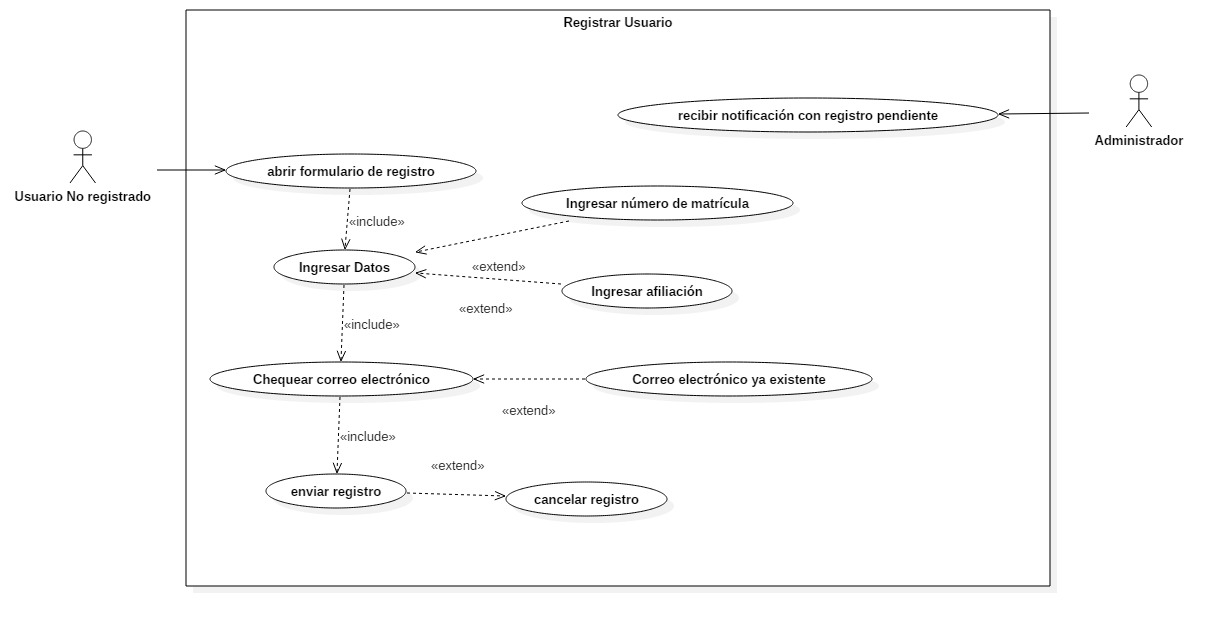
\includegraphics[width=\textwidth]{images/usecase/PUC01}
\label{FIG:CU_PUC01}
\caption{Diagrama de caso de uso para PUC01: Registrar usuario}
\end{figure}

\begin{figure}[!ht]
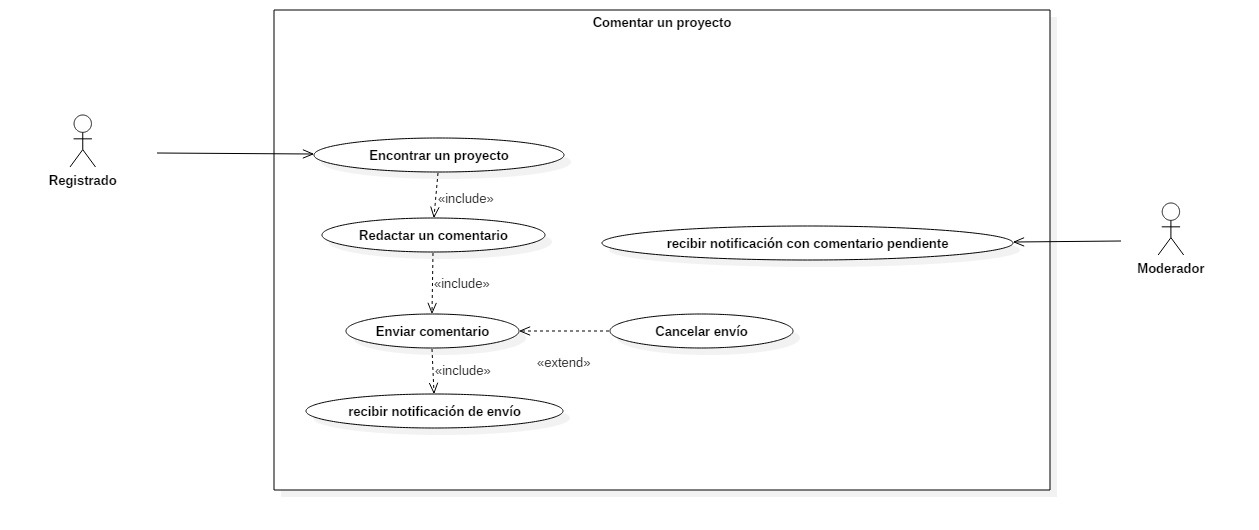
\includegraphics[width=\textwidth]{images/usecase/PUC02}
\label{FIG:CU_PUC02}
\caption{Diagrama de caso de uso para PUC02: Comentar un proyecto}
\end{figure}

\begin{figure}[!ht]
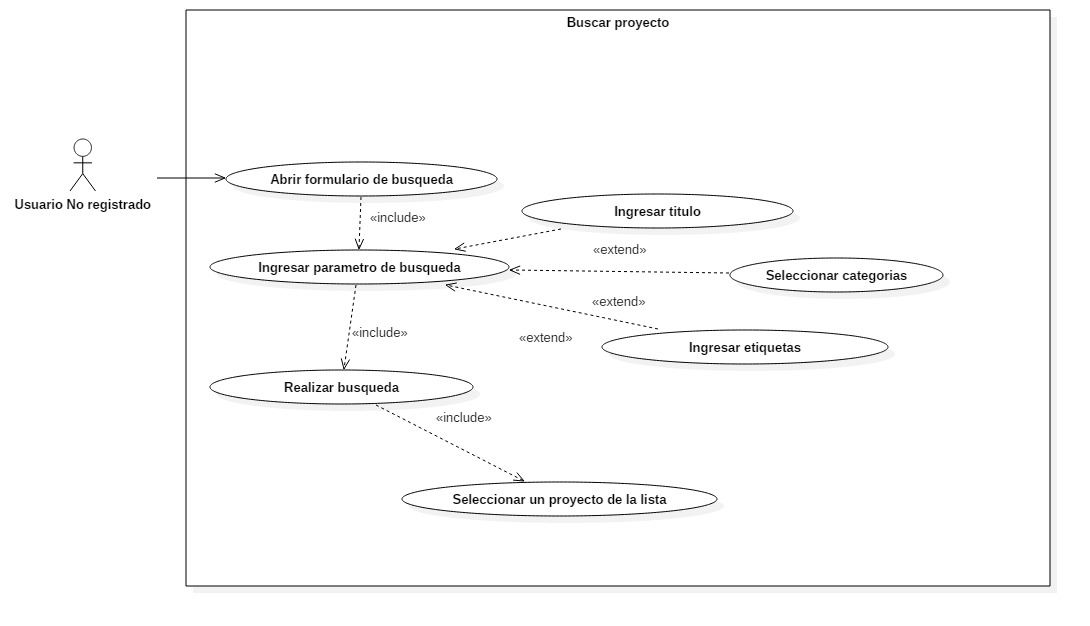
\includegraphics[width=\textwidth]{images/usecase/PUC03}
\label{FIG:CU_PUC03}
\caption{Diagrama de caso de uso para PUC03: Buscar proyecto}
\end{figure}

\begin{figure}[!ht]
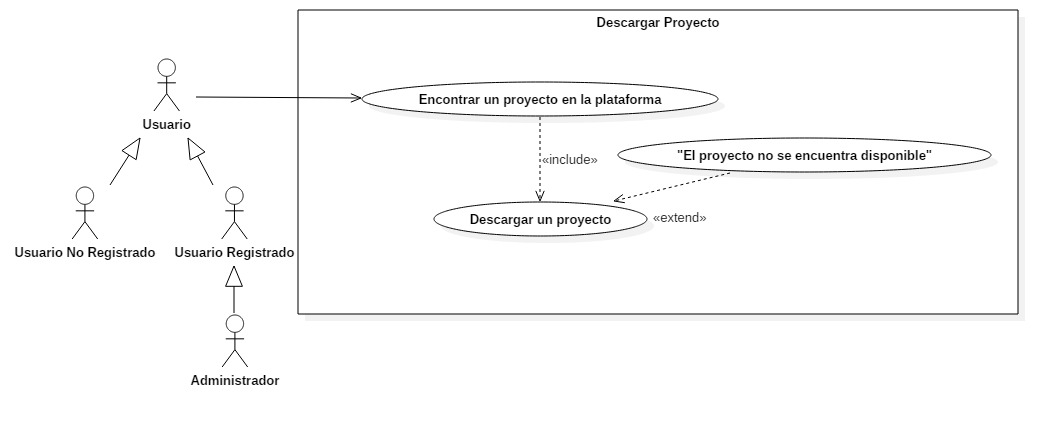
\includegraphics[width=\textwidth]{images/usecase/PUC04}
\label{FIG:CU_PUC04}
\caption{Diagrama de caso de uso para PUC04: Descargar Proyecto P\`ublico}
\end{figure}

\begin{figure}[!ht]
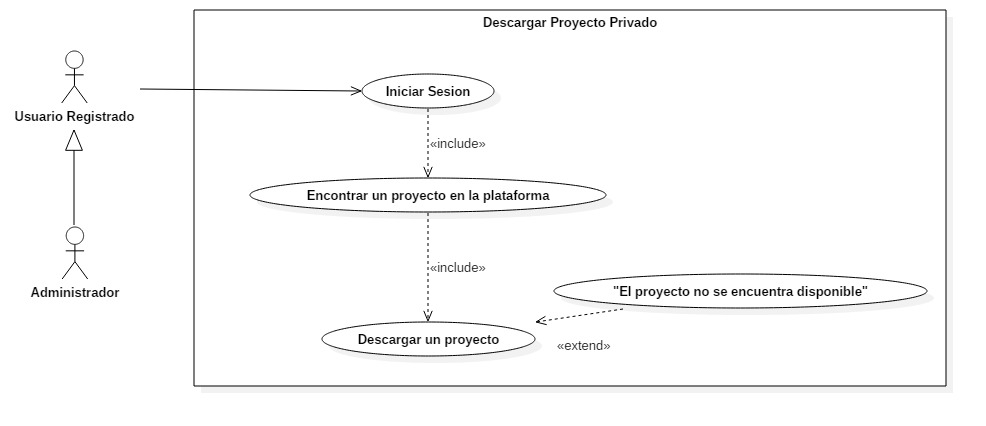
\includegraphics[width=\textwidth]{images/usecase/PUC05}
\label{FIG:CU_PUC05}
\caption{Diagrama de caso de uso para PUC05: Descargar Proyecto Privado}
\end{figure}

\begin{figure}[!ht]
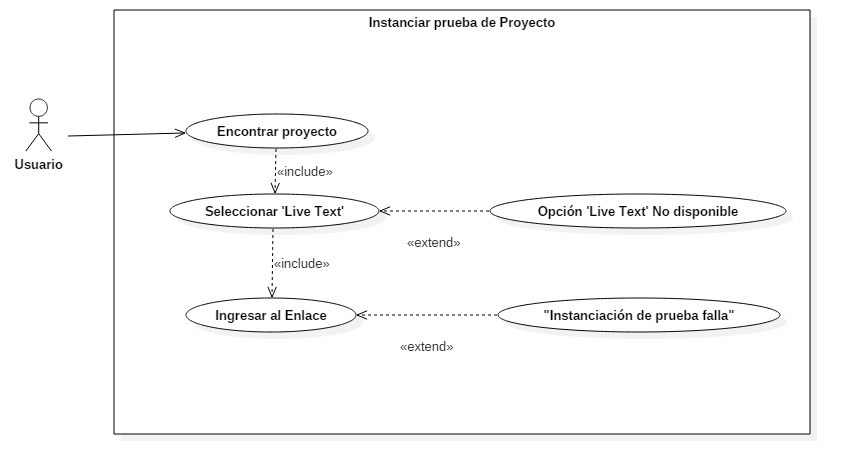
\includegraphics[width=\textwidth]{images/usecase/PUC06}
\label{FIG:CU_PUC06}
\caption{Diagrama de caso de uso para PUC06: Instanciar Prueba de Proyecto}
\end{figure}

\begin{figure}[!ht]
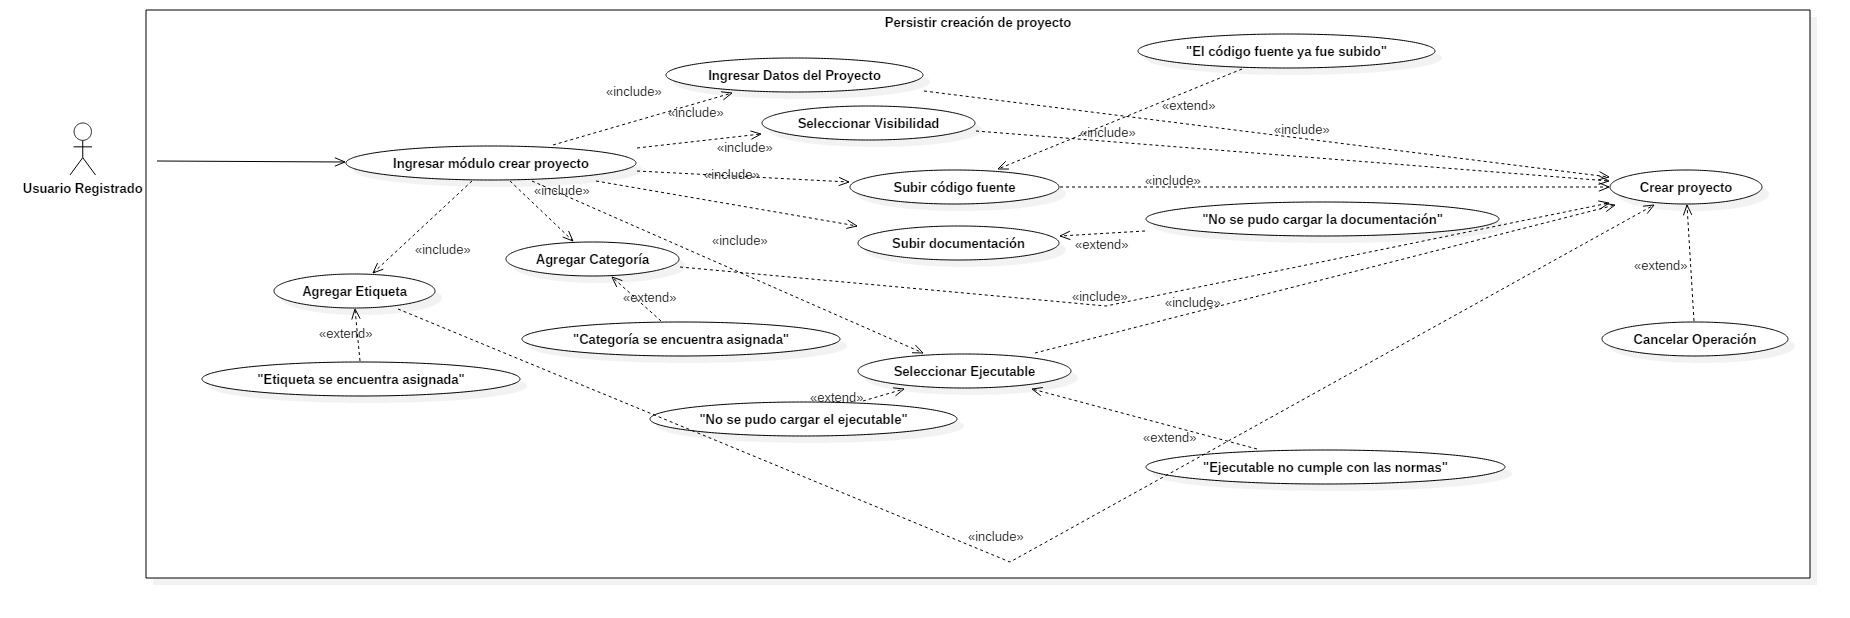
\includegraphics[width=\textwidth]{images/usecase/PUC07}
\label{FIG:CU_PUC07}
\caption{Diagrama de caso de uso para PUC07: Persistir creaci\'n de Proyecto}
\end{figure}

\begin{figure}[!ht]
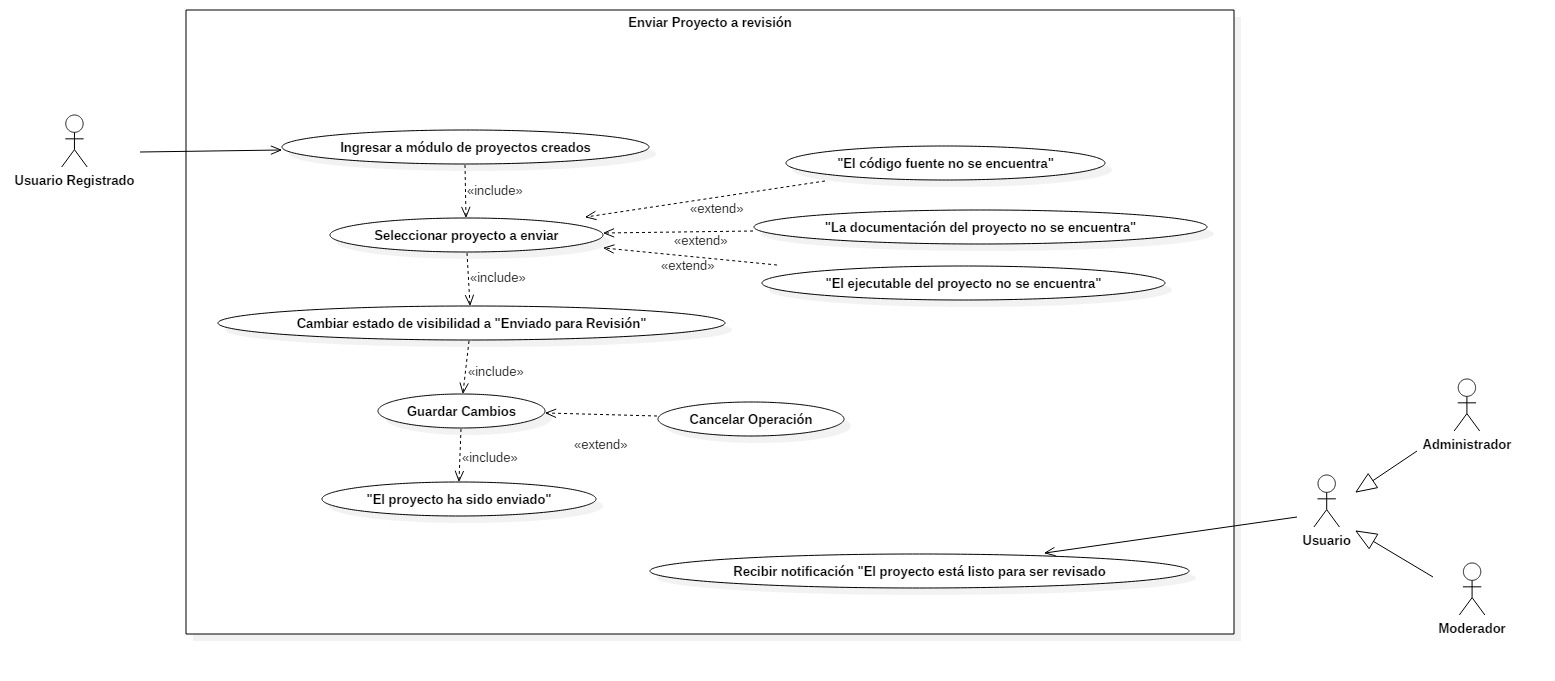
\includegraphics[width=\textwidth]{images/usecase/PUC08}
\label{FIG:CU_PUC08}
\caption{Diagrama de caso de uso para PUC08: Enviar proyecto a revisi\'n}
\end{figure}

\begin{figure}[!ht]
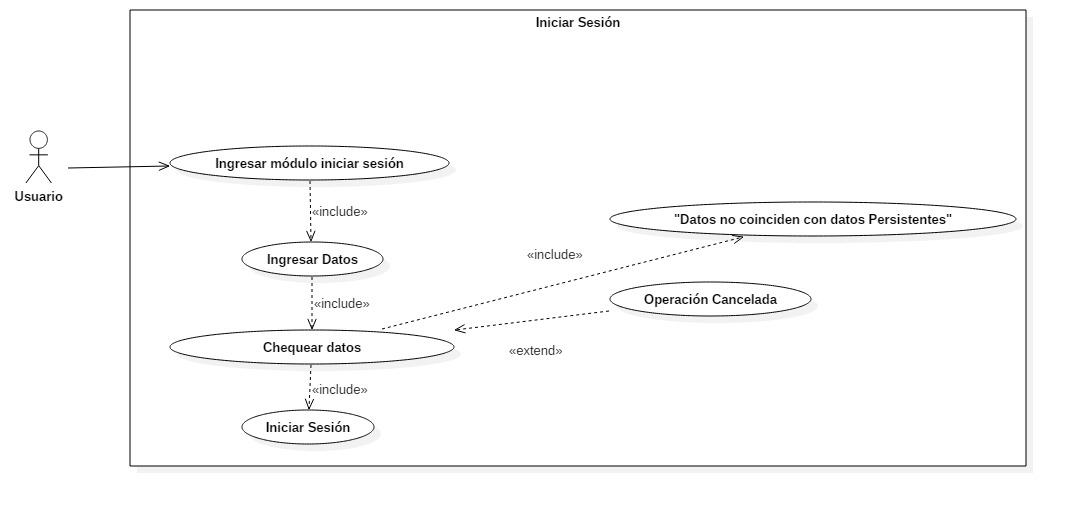
\includegraphics[width=\textwidth]{images/usecase/PUC09}
\label{FIG:CU_PUC09}
\caption{Diagrama de caso de uso para PUC09: Iniciar Sesi\`on}
\end{figure}

\begin{figure}[!ht]
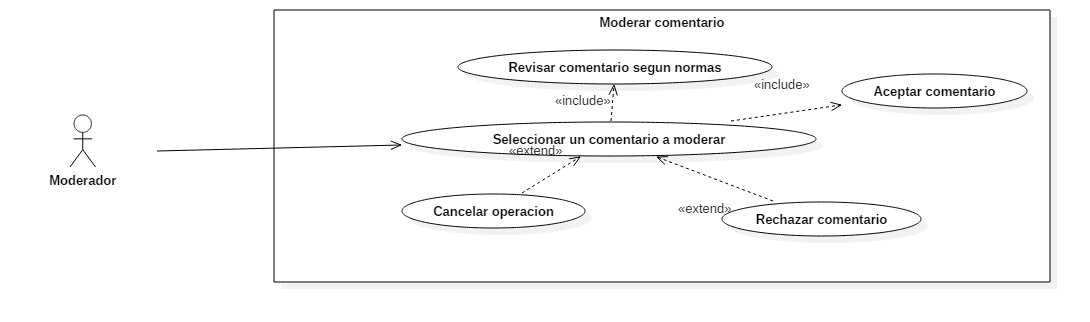
\includegraphics[width=\textwidth]{images/usecase/PUC10} %%falta PUC
\label{FIG:CU_PUC10}
\caption{Diagrama de caso de uso para PUC10: Moderar comentario}
\end{figure}

\begin{figure}[!ht]
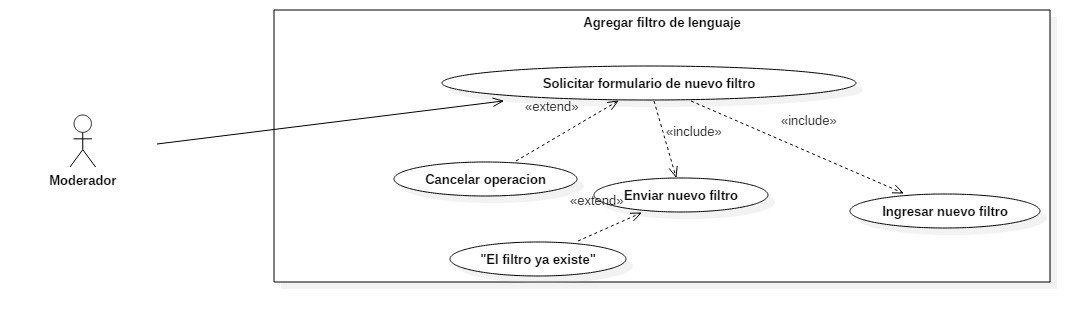
\includegraphics[width=\textwidth]{images/usecase/PUC11} %%falta PUC
\label{FIG:CU_PUC11}
\caption{Diagrama de caso de uso para PUC11: Agregar filtro de lenguaje}
\end{figure}

\begin{figure}[!ht]
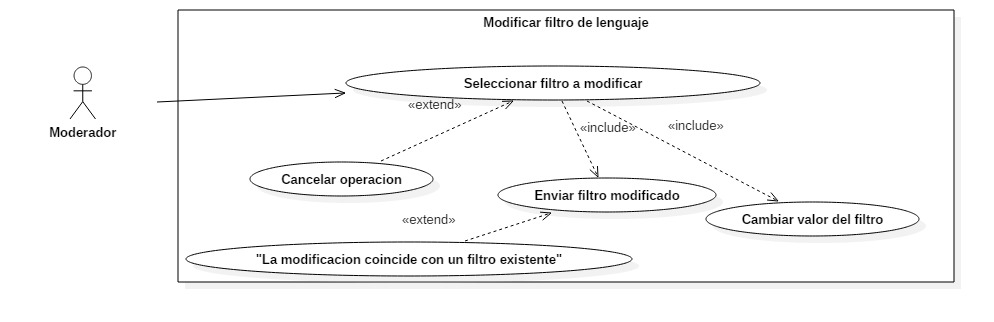
\includegraphics[width=\textwidth]{images/usecase/PUC12} %%falta PUC
\label{FIG:CU_PUC12}
\caption{Diagrama de caso de uso para PUC12: Modificar de filtro de lenguaje}
\end{figure}

\begin{figure}[!ht]
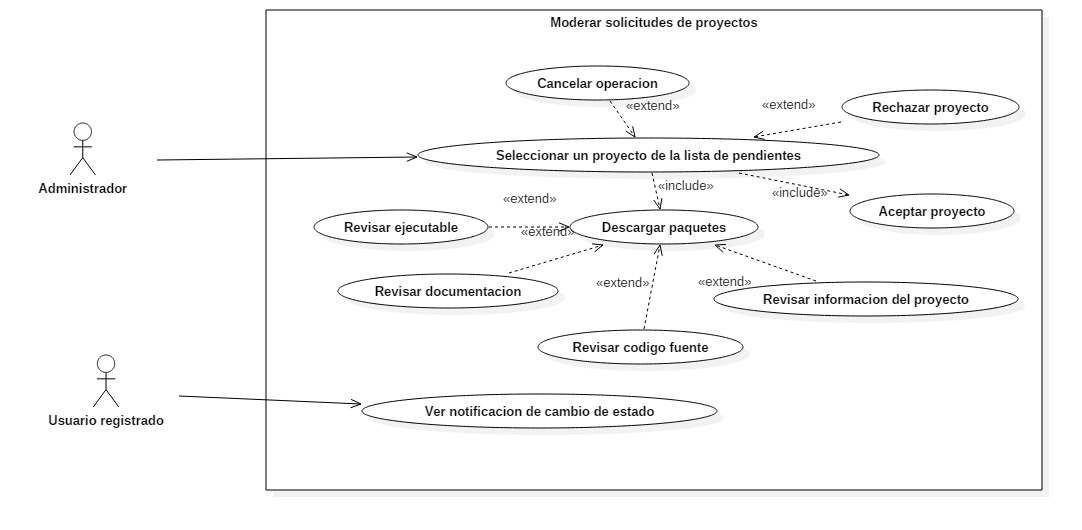
\includegraphics[width=\textwidth]{images/usecase/PUC13}
\label{FIG:CU_PUC13}
\caption{Diagrama de caso de uso para PUC13: Moderar proyectos}
\end{figure}

\begin{figure}[!ht]
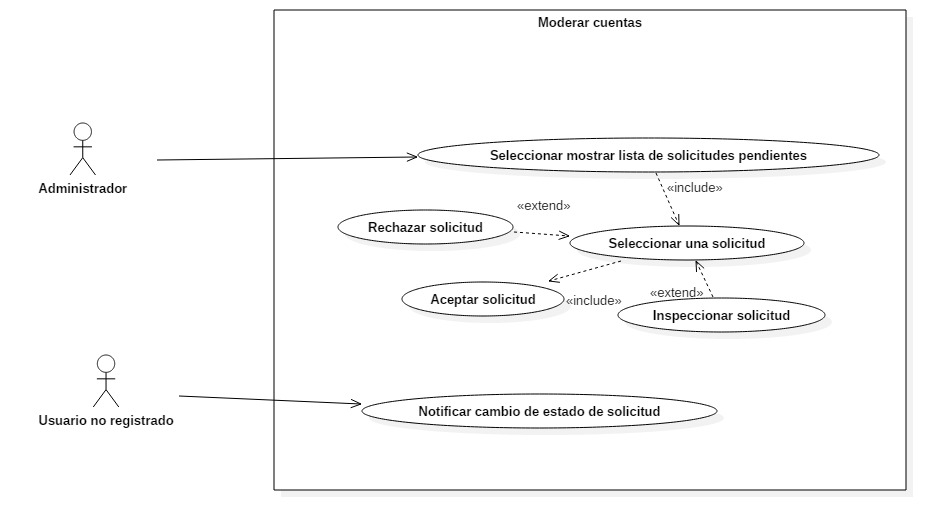
\includegraphics[width=\textwidth]{images/usecase/PUC14}
\label{FIG:CU_PUC14}
\caption{Diagrama de caso de uso para PUC14: Moderar cuentas}
\end{figure}

\begin{figure}[!ht]
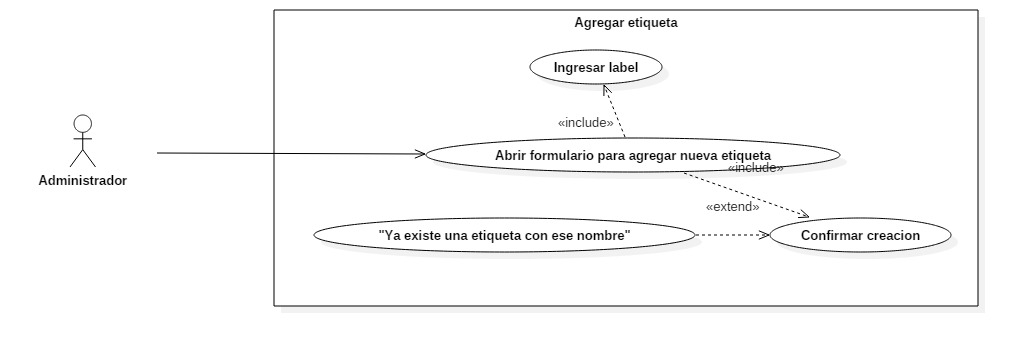
\includegraphics[width=\textwidth]{images/usecase/PUC15}
\label{FIG:CU_PUC15}
\caption{Diagrama de caso de uso para PUC15: Agregar una etiqueta}
\end{figure}

\begin{figure}[!ht]
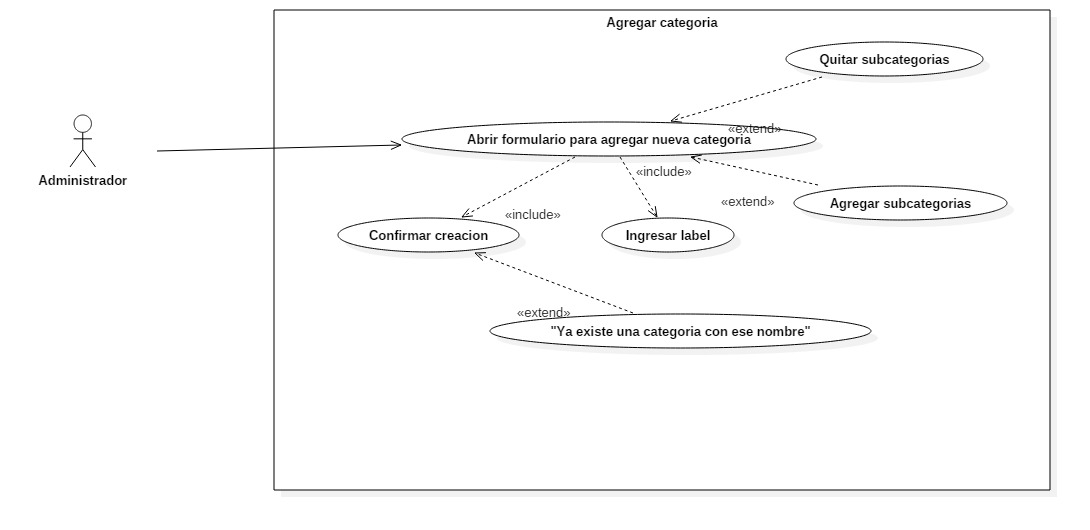
\includegraphics[width=\textwidth]{images/usecase/PUC16}
\label{FIG:CU_PUC16}
\caption{Diagrama de caso de uso para PUC16: Agregar una categor\`ia}
\end{figure}

\begin{figure}[!ht]
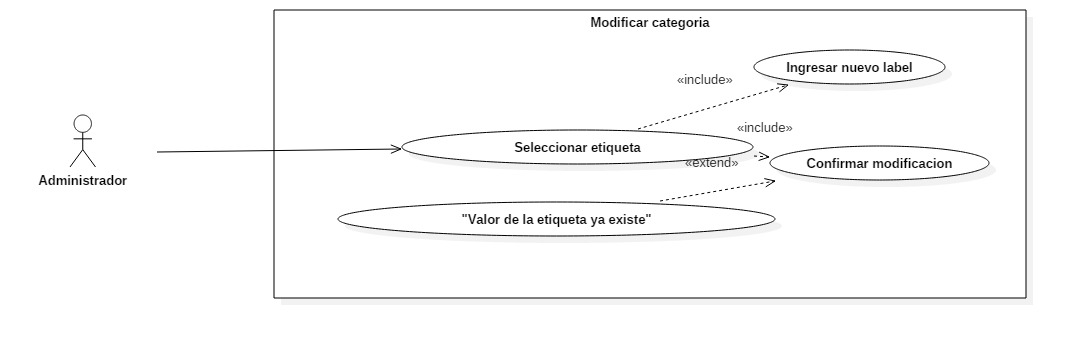
\includegraphics[width=\textwidth]{images/usecase/PUC17}
\label{FIG:CU_PUC17}
\caption{Diagrama de caso de uso para PUC17: Modificar una etiqueta}
\end{figure}
\clearpage
\begin{figure}[!ht]
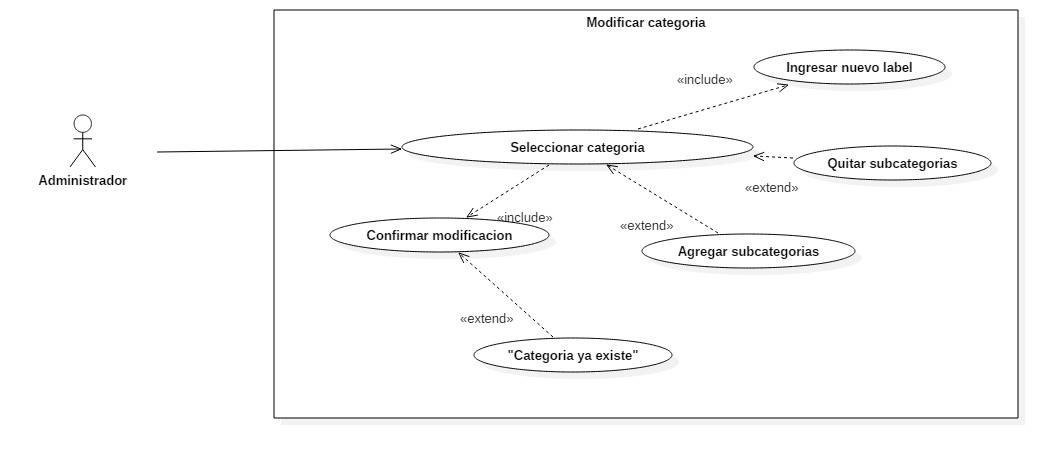
\includegraphics[width=\textwidth]{images/usecase/PUC18}
\label{FIG:CU_PUC18}
\caption{Diagrama de caso de uso para PUC18: Modificar una categor\`ia}
\end{figure}

\begin{figure}[!ht]
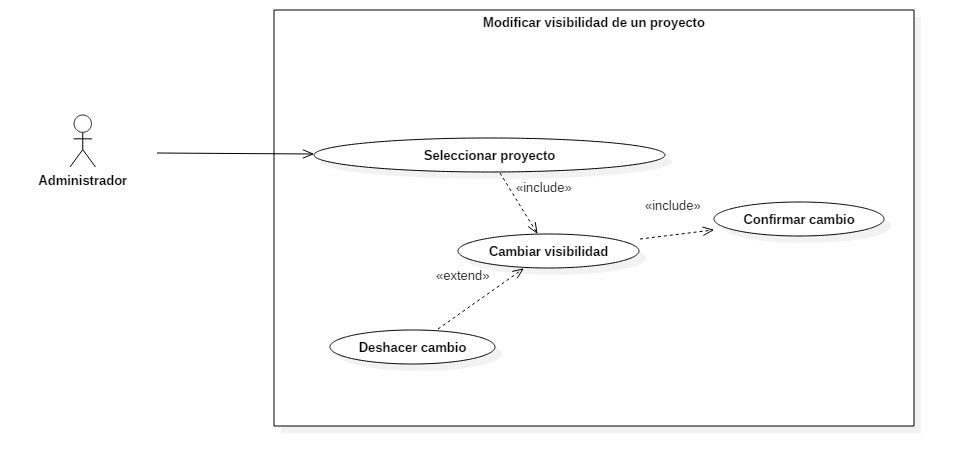
\includegraphics[width=\textwidth]{images/usecase/PUC19}
\label{FIG:CU_PUC19}
\caption{Diagrama de caso de uso para PUC19: Modificar Visibilidad de Proyecto}
\end{figure}

\begin{figure}[!ht]
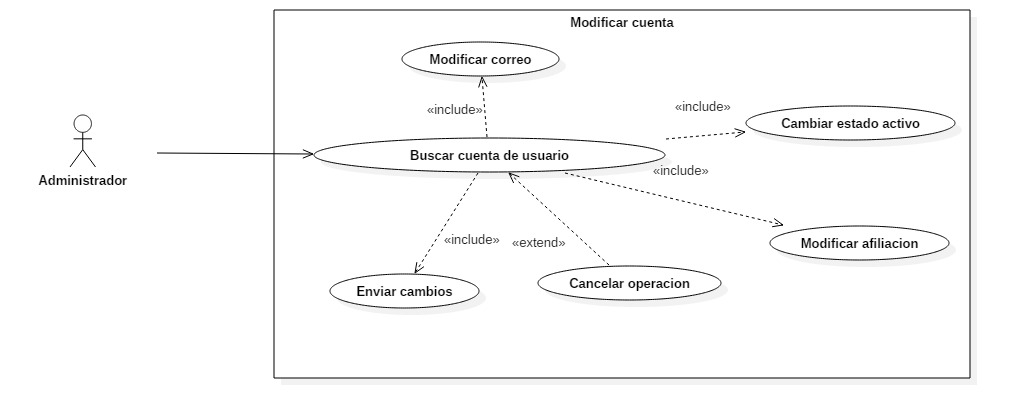
\includegraphics[width=\textwidth]{images/usecase/PUC20}
\label{FIG:CU_PUC20}
\caption{Diagrama de caso de uso para PUC20: Modificar cuenta}
\end{figure}

\begin{figure}[!ht]
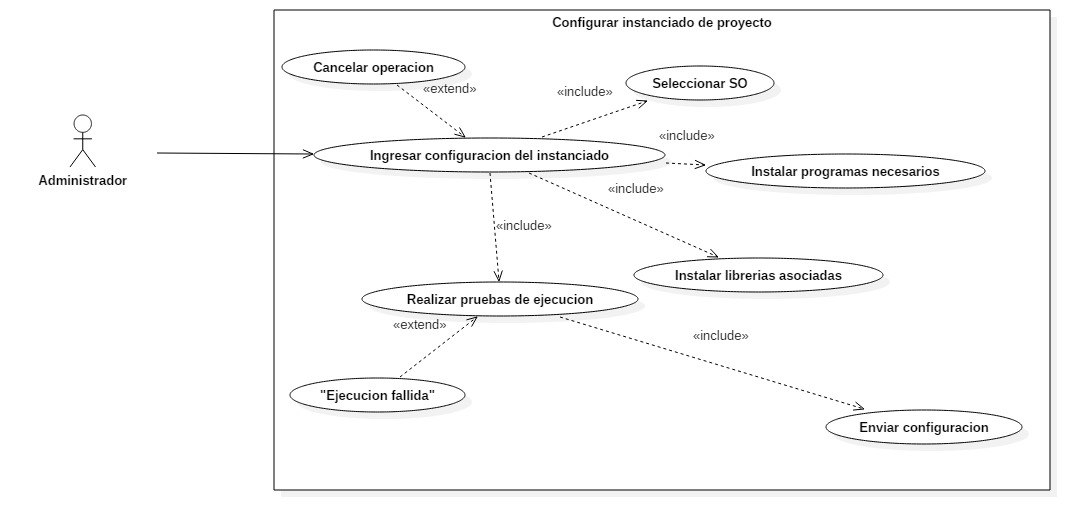
\includegraphics[width=\textwidth]{images/usecase/PUC21}
\label{FIG:CU_PUC21}
\caption{Diagrama de caso de uso para PUC21: Configurar instanciado de Proyecto}
\end{figure}

\begin{figure}[!ht]
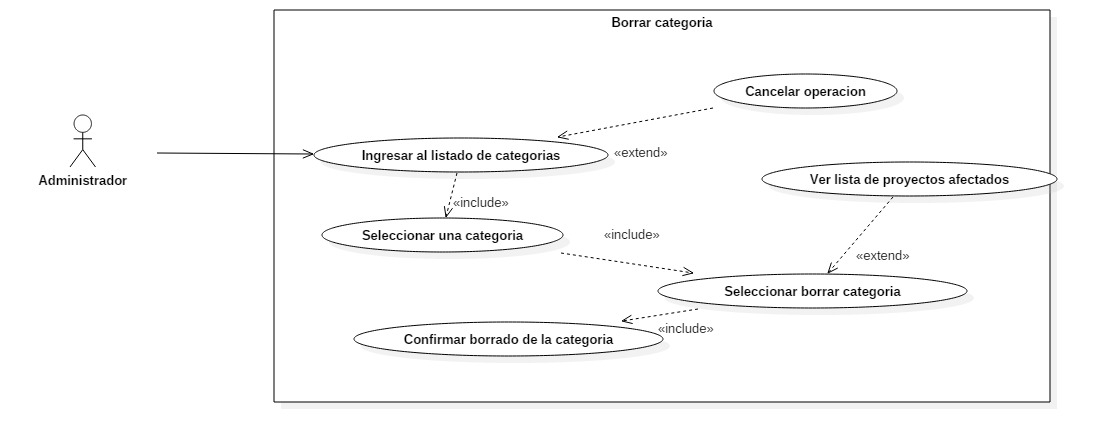
\includegraphics[width=\textwidth]{images/usecase/PUC22}
\label{FIG:CU_PUC22}
\caption{Diagrama de caso de uso para PUC22: Borrar categor\`ia}
\end{figure}

\begin{figure}[!ht]
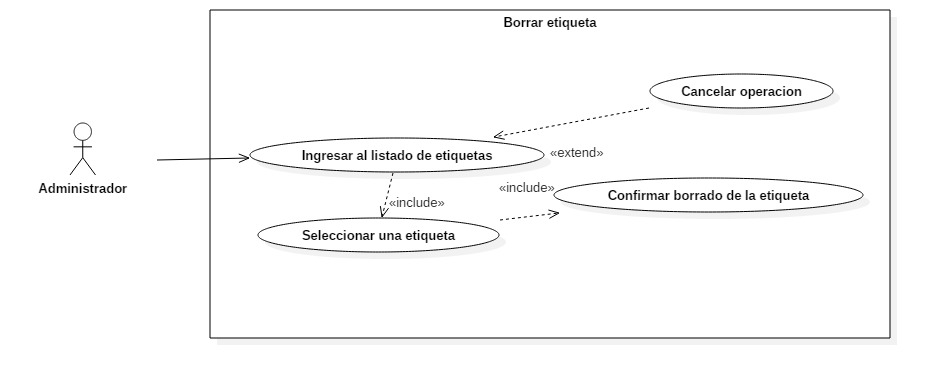
\includegraphics[width=\textwidth]{images/usecase/PUC23}
\label{FIG:CU_PUC23}
\caption{Diagrama de caso de uso para PUC23: Borrar etiqueta}
\end{figure}

\begin{figure}[!ht]
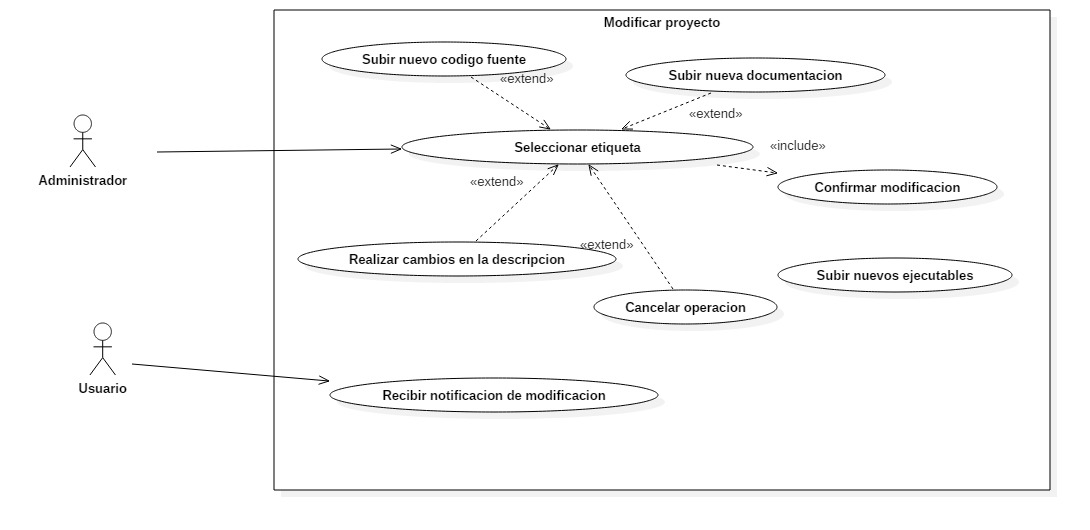
\includegraphics[width=\textwidth]{images/usecase/PUC24}
\label{FIG:CU_PUC24}
\caption{Diagrama de caso de uso para PUC24: Modificar Proyecto}
\end{figure}

\chapter{Prototipos}

\begin{figure}[!ht]

\includegraphics[width=\textwidth]{images/proto/1}
\label{FIG:PROTO_1}
\caption{Prototipo de pantalla de inicio}
\end{figure}

\begin{figure}[!ht]
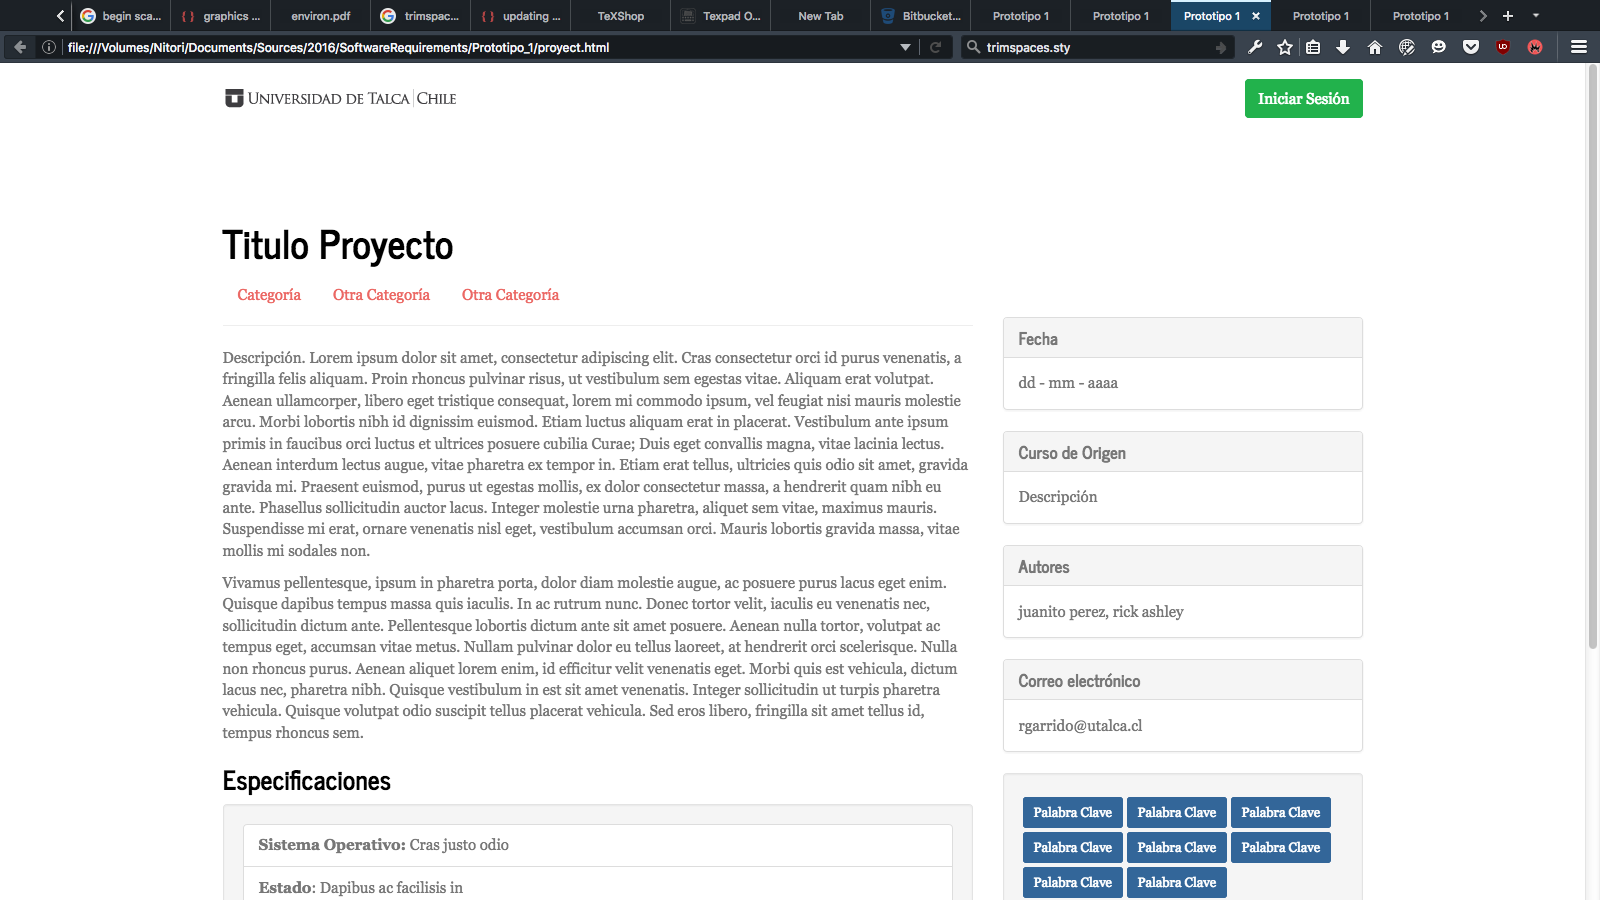
\includegraphics[width=\textwidth]{images/proto/2}
\label{FIG:PROTO_2}
\caption{Prototipo de vista de proyecto}
\end{figure}

\begin{figure}[!ht]
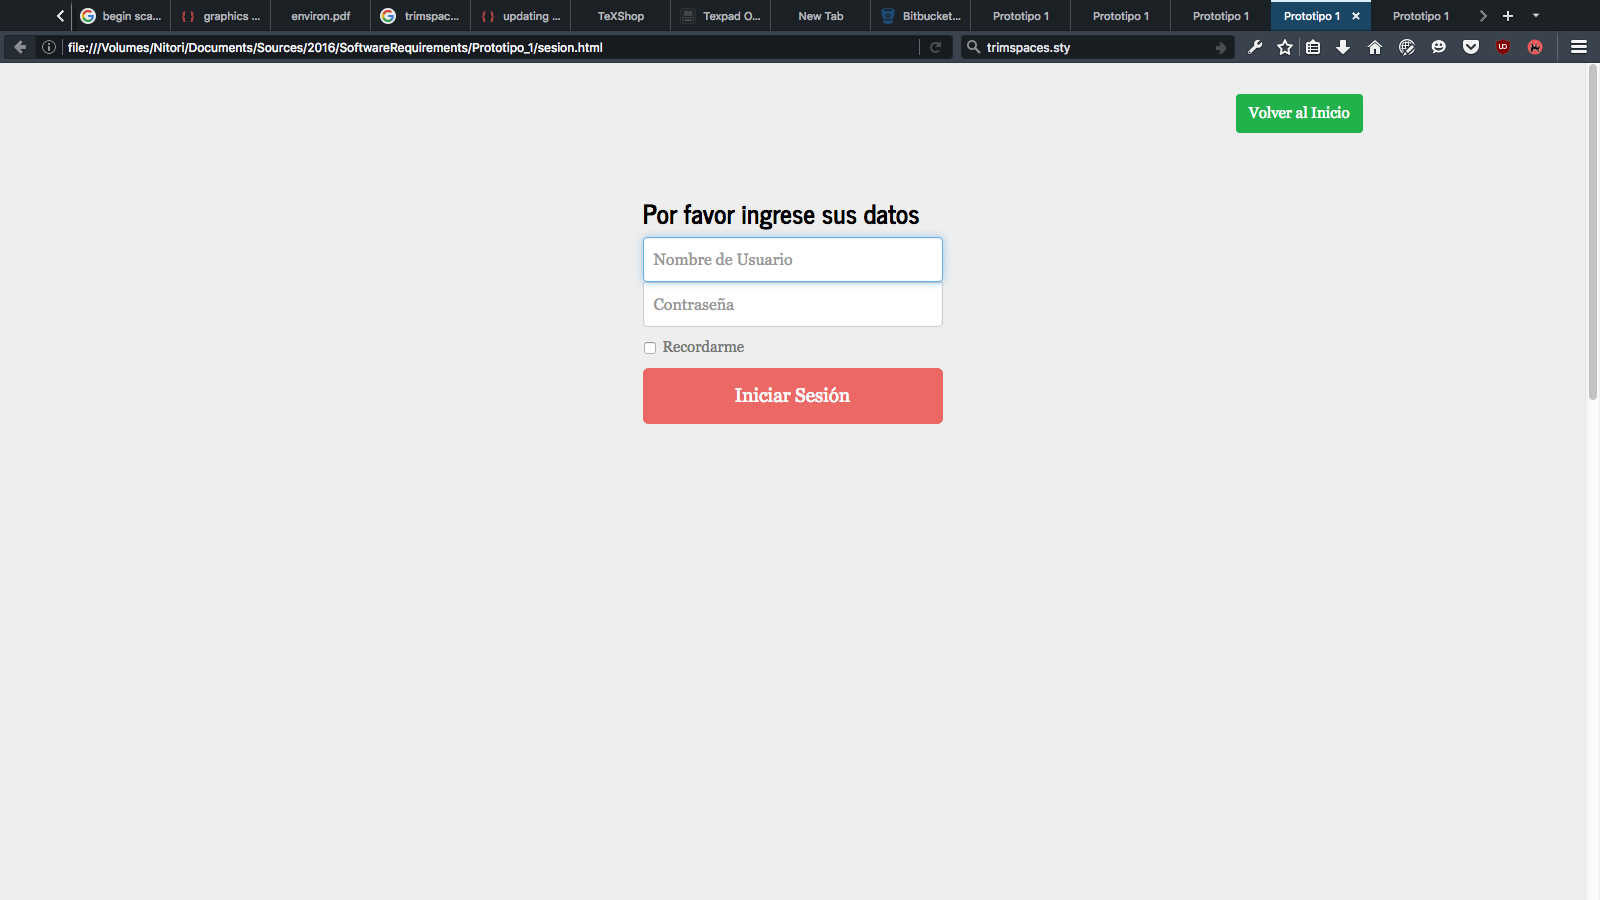
\includegraphics[width=\textwidth]{images/proto/3}
\label{FIG:PROTO_3}
\caption{Prototipo de pantalla de login}
\end{figure}

\begin{figure}[!ht]
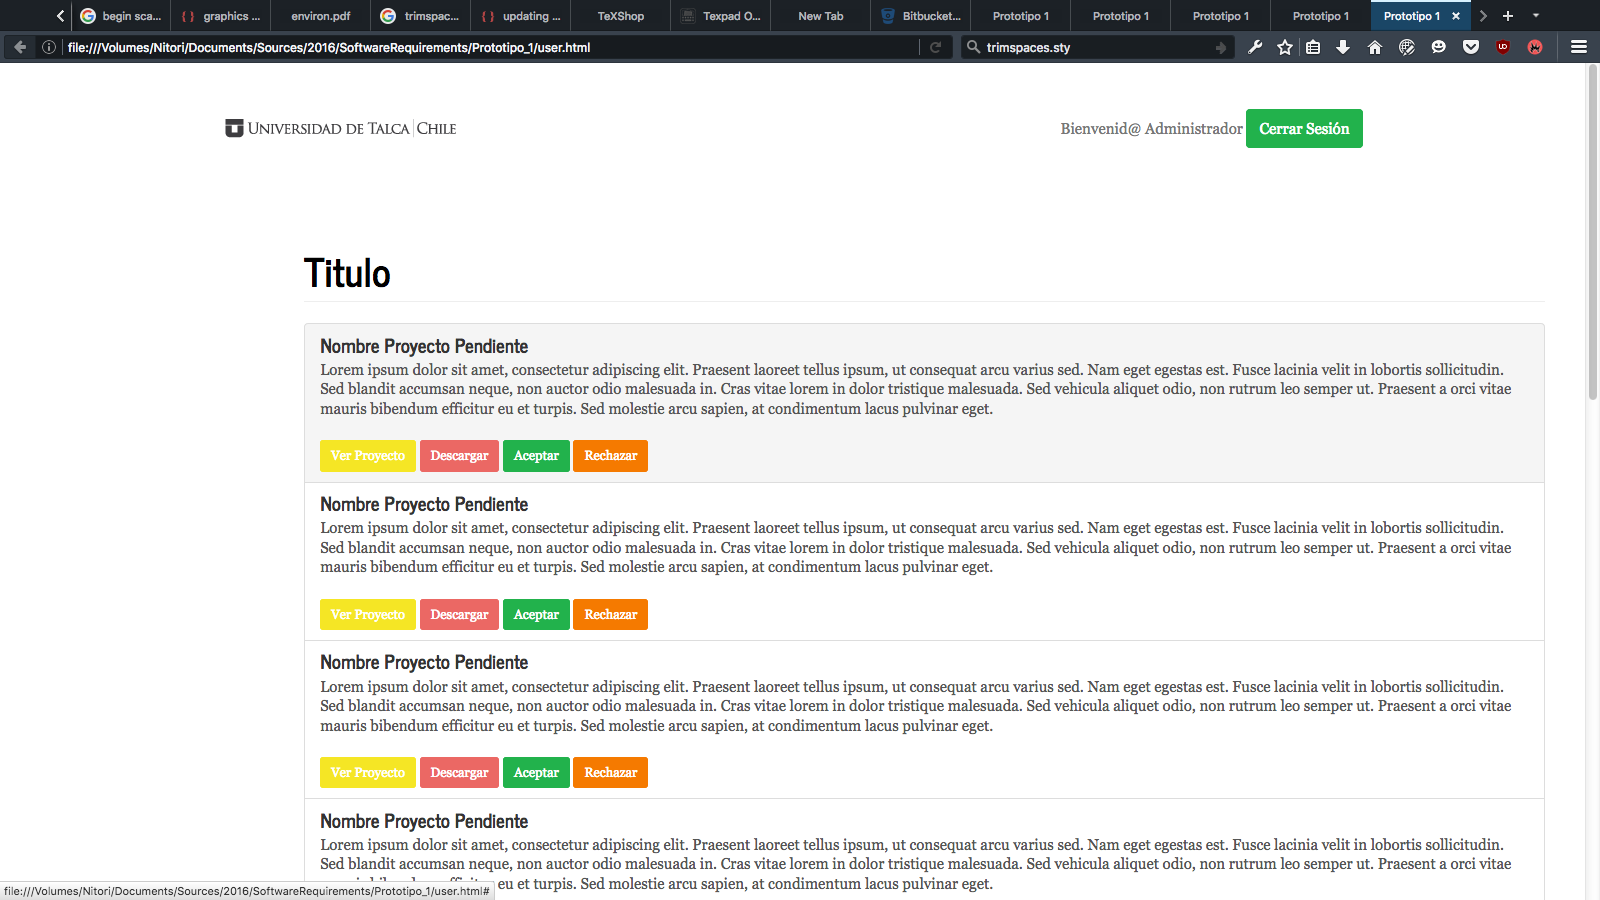
\includegraphics[width=\textwidth]{images/proto/4}
\label{FIG:PROTO_4}
\caption{Prototipo de lista de proyectos (admin)}
\end{figure}

\end{document}